\documentclass{ctexart}

\usepackage[margin=1in]{geometry}
\usepackage{setspace}
\usepackage{graphicx}
\usepackage{tabularx}
\usepackage{caption}
\usepackage{indentfirst}
\usepackage{titling}
\usepackage{multirow}
\usepackage{diagbox}
\usepackage{tikz}
\usepackage{subcaption}
\usepackage{float}
\usepackage{multicol}
\usepackage{blindtext}
\usepackage{pdfpages}
\usepackage{hyperref}
\usepackage{siunitx}
\usepackage{textcomp,mathcomp}
\usepackage{amsmath}
\usepackage{booktabs}
\usepackage{listings}
\usepackage{color}
\usepackage{cite}
\lstset{
    language=Python,
    backgroundcolor=\color{gray!10},
    basicstyle=\ttfamily\footnotesize,
    numbers=left,
    numberstyle=\tiny\color{gray},
    keywordstyle=\color{blue},
    commentstyle=\color{dkgreen},
    stepnumber=1,
    numbersep=5pt,
    showspaces=false,
    showstringspaces=false,
    showtabs=false,
    frame=single,
    rulecolor=\color{black},
    tabsize=4,
    captionpos=b,
    breaklines=true, % 启用自动换行
    breakatwhitespace=false,
    title=\lstname
}

\preauthor{\begin{flushleft}}
\postauthor{\end{flushleft}}

\title{HIV感染模型及药物疗效分析的可视化}
\date{}
\author{\qquad \\ \textbf{\Large{张凌诚} }PB22081589 \\中国科学技术大学生物科学系,合肥 \textbf{230026} \\联系人,\textbf{E-mail:} \href{zlc2208@mail.ustc.edu.cn}{zlc2208@mail.ustc.edu.cn}}

\begin{document}
\maketitle
\begin{titlepage}
    \tableofcontents
\end{titlepage}

\section{科学技术原理}
\subsection{问题背景}
人类免疫缺陷病毒(Human Immunodeficiency Virus, HIV)是造成人类免疫系统缺陷的一种逆转录病毒。其主要攻击并逐渐破坏人类的免疫系统,致使宿主死于其他病原体的继发感染或者自身癌变细胞的扩散。而艾滋病就是HIV感染的最后阶段免疫力丧失症状的总称。建立HIV的感染模型并且通过数值模拟模型对不同药物的响应,有助于优化针对HIV感染的多药物联合治疗方案。而将计算结果可视化,有助于我们直观地了解模型的动力学特性。

\subsection{HIV感染模型的建立}
这里我们选择了“包含潜伏感染阶段的具有两种靶细胞的HIV感染模型”\cite{1}进行感染过程和药物疗效的可视化。该模型考虑HIV感染两种免疫细胞$CD4^{+}T$细胞($T_{1}$)和巨噬细胞($T_{2}$),每种细胞分别有未感染(T)、感染(I)以及潜伏感染(L)三种状态\cite{3};同时由于逆转录酶抑制剂($\varepsilon _{RT}$)和蛋白酶抑制剂($\varepsilon _{PI}$)的作用\cite{2},胞外病毒颗粒也可以分为有感染性($V_{I}$)和无感染性($V_{NI}$)两类。

\paragraph{未感染细胞的变化率($\dot{T} $):}等于未感染细胞的产生速率($\lambda $)减去未感染细胞死亡速率($d_{T}T$),再减去病毒感染速率($\beta (1-\varepsilon _{RT})TV_{I}$),即:
$$\dot{T}=\lambda-d_{T}T-\beta (1-\varepsilon _{RT})TV_{I}$$
其中$\lambda$为未感染细胞的产生速率,$d_{T}$为未感染细胞死亡率,$\beta $为病毒感染率,$\varepsilon _{RT}$为逆转录酶抑制剂\footnote{可以降低免疫细胞的病毒感染率。}药效。

\paragraph{潜伏感染细胞变化率($\dot{L}$):}等于感染病毒的细胞进入潜伏期的速率($f\beta (1-\varepsilon _{RT})TV_{I}$)减去潜伏感染细胞转为感染期的速率($\alpha L$),再减去潜伏感染细胞的死亡速率($\delta _{L}L$),即:
$$\dot{L}=f\beta (1-\varepsilon _{RT})TV_{I}-\alpha L-\delta _{L}L$$
其中$f$为感染病毒的细胞转为潜伏感染细胞比例,$\alpha$为潜伏感染细胞的激活率,$\delta _{L}$为潜伏感染细胞死亡率。

\paragraph{感染细胞的变化率($\dot{I}$):}等于感染病毒的细胞进入感染期的速率($(1-f)\beta (1-\varepsilon _{RT})TV_{I}$)加上潜伏感染细胞转为感染期的速率($\alpha L$),再减去感染细胞的死亡速率($\delta _{I}I$),即
$$\dot{I}=(1-f)\beta (1-\varepsilon _{RT})TV_{I}+\alpha L-\delta _{I}I$$
其中$\delta _{I}$为感染细胞死亡率。

\paragraph{胞外有感染性毒粒变化率($\dot{V}_{I}$):}等于感染细胞死亡后感染性病毒裂解量($N(1-\varepsilon _{PI})$)乘感染细胞的死亡速率($\delta _{I}I$)即为胞外感染性病毒产生速率,再减去胞外感染性病毒清除速率($c_{V}V_{I}$),即
$$\dot{V}_{I}=N(1-\varepsilon _{PI})\delta _{I}I-c_{V}V_{I}$$
其中$N$为感染细胞内病毒的裂解量,$\varepsilon _{PI}$为蛋白酶抑制剂\footnote{可以抑制病毒感染能力,使部分毒粒失去感染能力。}药效,$c_{V}$为病毒清除率。

\paragraph{胞外感染性毒粒变化率($\dot{V}_{NI}$):}等于感染细胞死亡后无感染性病毒裂解量($N\varepsilon _{PI}$)乘感染细胞的死亡速率($\delta _{I}I$)即为胞外无感染性病毒产生速率,再减去胞外无感染性病毒清除速率($c_{V}V_{NI}$),即
$$\dot{V}_{NI}=N\varepsilon _{PI}\delta _{I}I-c_{V}V_{NI}$$

\paragraph{“两种靶细胞的HIV感染模型”:}考虑到HIV主要感染$CD4^{+}T$细胞($T_{1}$)和巨噬细胞($T_{2}$)两种靶细胞,其感染的动力学过程基本相同,但微分方程的相关参数不尽相同(表\ref{tab.1}),故仅以下标$ _{1}, _{2}$作为区分。合并上述一阶微分方程得:
$$\left\{
    \begin{aligned}
        \dot{T}_{1}  & =\lambda_{1}-d_{T_{1}}T_{1}-\beta_{1} (1-\varepsilon _{1RT})T_{1}V_{I}                                       \\
        \dot{L}_{1}  & =f_{1}\beta_{1} (1-\varepsilon _{1RT})T_{1}V_{I}-\alpha_{1} L_{1}-\delta _{L_{1}}L_{1}                       \\
        \dot{I}_{1}  & =(1-f_{1})\beta_{1} (1-\varepsilon _{1RT})T_{1}V_{I}+\alpha_{1} L_{1}-\delta _{I_{1}}I_{1}                   \\
        \dot{T}_{2}  & =\lambda_{2}-d_{T_{2}}T_{2}-\beta_{2} (1-\varepsilon _{2RT})T_{2}V_{I}                                       \\
        \dot{L}_{2}  & =f_{2}\beta_{2} (1-\varepsilon _{2RT})T_{2}V_{I}-\alpha_{2} L_{2}-\delta _{L_{2}}L_{2}                       \\
        \dot{I}_{2}  & =(1-f_{2})\beta_{2} (1-\varepsilon _{2RT})T_{2}V_{I}+\alpha_{2} L_{2}-\delta _{I_{2}}I_{2}                   \\
        \dot{V}_{I}  & =N_{1}(1-\varepsilon _{1PI})\delta _{I_{1}}I_{1}+N_{2}(1-\varepsilon _{2PI})\delta _{I_{2}}I_{2}-c_{1V}V_{I} \\
        \dot{V}_{NI} & =N_{1}\varepsilon _{1PI}\delta _{I_{1}}I_{1}+N_{2}\varepsilon _{2PI}\delta _{I_{2}}I_{2}-c_{2V}V_{NI}
    \end{aligned}
    \right.$$

\begin{table}[H]
    \centering
    \caption{微分方程组参数表}
    \label{tab.1}
    \begin{tabular}{clclclclcl}
        \toprule
        参数                                                       & 含义                        & 单位                        & 取值                  & 参考        \\
        \midrule
        $\lambda _{1}$                                           & 未感染$CD4^{+}T$细胞产生速率       & $mm^{-3}day^{-1}$         & 10                  & \cite{4}  \\
        $\lambda _{2}$                                           & 未感染巨噬细胞产生速率               & $mm^{-3}day^{-1}$         & 0.04                & \cite{5}  \\
        $d_{T_{1}}$                                              & 未感染$CD4^{+}T$细胞死亡率        & $day^{-1}$                & 0.01                & \cite{4}  \\
        $d_{T_{2}}$                                              & 未感染巨噬细胞细胞死亡率              & $day^{-1}$                & 0.01                & \cite{5}  \\
        \textcolor{red}{$\beta_{1}$}                             & $CD4^{+}T$细胞病毒感染率         & $mm^{3}day^{-1}$          & $\num{e-5}\sim 0.5$ & \cite{7}  \\
        \textcolor{red}{$\beta_{2}$}                             & 巨噬细胞病毒感染率                 & $mm^{3}day^{-1}$          & $\num{e-5}\sim 0.5$ & \cite{7}  \\
        $f_{1}$                                                  & 感染的$CD4^{+}T$细胞转化为潜伏感染的比例 & -                         & 0.1                 & \cite{8}  \\
        $f_{2}$                                                  & 感染的巨噬细胞转化为潜伏感染的比例         & -                         & 0.1                 & \cite{8}  \\
        $\alpha_{1}$                                             & 潜伏感染$CD4^{+}T$细胞激活率       & $day^{-1}$                & 0.2                 & \cite{9}  \\
        $\alpha_{2}$                                             & 潜伏感染巨噬细胞激活率               & $day^{-1}$                & 0.05                & \cite{10} \\
        $\delta_{L_{1}}$                                         & 潜伏感染$CD4^{+}T$细胞死亡率       & $day^{-1}$                & 0.02                & \cite{10} \\
        $\delta_{L_{2}}$                                         & 潜伏感染巨噬细胞死亡率               & $day^{-1}$                & 0.1                 & \cite{10} \\
        $\delta_{I_{1}}$                                         & 感染$CD4^{+}T$细胞死亡率         & $day^{-1}$                & 0.5                 & \cite{11} \\
        $\delta_{I_{2}}$                                         & 感染巨噬细胞死亡率                 & $day^{-1}$                & 0.1                 & \cite{11} \\
        $N_{1}$                                                  & $CD4^{+}T$细胞内病毒裂解量        & $virions\quad cells^{-1}$ & 15                  & \cite{10} \\
        $N_{2}$                                                  & 巨噬细胞内病毒裂解量                & $virions\quad cells^{-1}$ & 10                  & \cite{11} \\
        $c_{1V},c_{2V}$                                          & 胞外病毒清除速率                  & $day^{-1}$                & 3                   & \cite{4}  \\
        \textcolor{red}{$\varepsilon _{1RT},\varepsilon _{2RT}$} & 逆转录酶抑制剂抑制率                & -                         & (0,1)               & -         \\
        \textcolor{red}{$\varepsilon _{1PI},\varepsilon _{2PI}$} & 蛋白酶抑制剂抑制率                 & -                         & (0,1)               & -         \\
        \bottomrule
    \end{tabular}
\end{table}

\subsection{模型平衡点}
\subsubsection{无病平衡点}
无病平衡点即完全痊愈的情况,令方程组左边一阶微分全部为零且$V_{I}=0$,解得无病平衡点:
$$E^{0}=\left(T_{1}=\frac{\lambda_{1}}{d_{T_{1}}},L_{1}=0,I_{1}=0,T_{2}=\frac{\lambda_{2}}{d_{T_{2}}},L_{2}=0,I_{2}=0,V_{I}=0,V_{NI}=0\right) $$

\subsubsection{基本再生数$R_{0}$}
若不限制$V_{I}=0$,即在一般情况下求解稳态解,可得中间变量$$R_{0}=\frac{N_{1}(1-\varepsilon _{1PI})\beta_{1}(1-\varepsilon _{1RT})[\alpha_{1}+(1-f_{1})\delta_{L_{1}}]\lambda _{1}}{(\delta _{L_{1}}+\alpha_{1})c_{1V}d_{T_{1}}}+\frac{N_{2}(1-\varepsilon _{2PI})\beta_{2}(1-\varepsilon _{2RT})[\alpha_{2}+(1-f_{2})\delta_{L_{2}}]\lambda _{2}}{(\delta _{L_{2}}+\alpha_{2})c_{2V}d_{T_{2}}}$$定义$R_{0}$为基本再生数,表示每个HIV病毒的存活期间所能感染健康$CD4^{+}T$细胞和健康巨噬细胞的平均数量,其取值决定了最终的感染状态\cite{1}。从表\ref{tab.1}中可以发现一般情况下仅有$\beta_{1},\beta_{2},\varepsilon _{1RT},\varepsilon _{2RT},\varepsilon _{1PI},\varepsilon _{2PI}$六个参数为变量,所以可知:$$R_{0}(\beta_{1},\beta_{2},\varepsilon _{1RT},\varepsilon _{2RT},\varepsilon _{1PI},\varepsilon _{2PI})$$即HIV感染患者最终的感染状态由两种免疫细胞($CD4^{+}T$细胞和巨噬细胞)各自的感染率以及两种药物(逆转录酶抑制剂和蛋白酶抑制剂)的抑制率相关。

$\beta_{1},\beta_{2}$往往由病毒亚型和患者自身状态所决定不易改变,我们所关注的便是提高$\varepsilon _{RT},\varepsilon _{PI}$或是采用不同药物组合的联合疗法,控制$R_{0}$以控制最终感染状态。

\section{设计方案及程序结构}
\paragraph{python程序结构框架(设计方案)}:
\begin{enumerate}
    \item 实现单次感染过程的数值模拟;
    \item 对数值模拟方法进行精确度检验;
    \item 多次计算感染过程,积累绘图数据;
    \item 可视化感染过程及可变参数对终态的影响。
\end{enumerate}
\subsection{数值模拟单次感染过程}
\subsubsection{创建父类Cell}
创建类Cell在初始方法中通过列表params传入可变参数($\beta_{1},\beta_{2},\varepsilon _{1RT},\varepsilon _{2RT},\varepsilon _{1PI},\varepsilon _{2PI}$),同时传入数值模拟感染过程进行的时间($t_{e}$)和问题规模($n_{t}$)以计算时间微分($\delta t$)。设定HIV感染模型中的恒定参数($\alpha_{1},\alpha_{2},d_{T_{1}},d_{T_{2}}$等),并且用数组$cell\_process$来储存数值模拟过程中细胞浓度的变化。
\begin{lstlisting}[label={lst.1}, caption={父类Cell的参数、初始化条件及类方法}]
    class Cell:
    def __init__(self,params=[0.0001,0.015,0,0,0,0],te=1000,nt=10000):
        self.l1, self.l2 = 10, 0.04
        self.dT1, self.dT2 = 0.01, 0.01
        self.f1, self.f2 = 0.1, 0.1
        self.a1, self.a2 = 0.2, 0.05
        self.dL1, self.dL2 = 0.02, 0.1
        self.dI1, self.dI2 = 0.5, 0.1
        self.N1, self.N2 = 15, 10
        self.c1V, self.c2V = 3, 3
        self.b1, self.b2, self.e1RT, self.e2RT, self.e1PI, self.e2PI=params
        self.cell_process = np.zeros(int(nt+1))
        self.dt=te/nt

    def dnumber(self, T1=None, L1=None, I1=None, T2=None, L2=None, I2=None, VI=None, VNI=None, i=0):

    def process(self, T1=None, L1=None, I1=None, T2=None, L2=None, I2=None, VI=None, VNI=None, i=0):
        self.cell_process[i+1]=(self.cell_process[i] + self.dnumber(T1, L1, I1, T2, L2, I2, VI, VNI, i)*self.dt)

    def R0(self,params=[0.0001,0.015,0,0,0,0]):
\end{lstlisting}
类Cell中定义了三个类方法:
\begin{enumerate}
    \item dnumber():传入各子类的对象和循环变量(i)以计算循环(i)次时的细胞浓度变化速率。
    \item process():传入各子类的对象和循环变量(i),同时调用类方法dnumber,通过公式:$$cell[i+1]=cell[i]+\dot{cell}[i]\cdot \delta t$$即视细胞浓度变化过程为一个离散数组,在给定初始值的情况下通过递推求和,依次计算给定范围内元素的值。
    \item R0():根据传入的列表params=[$\beta_{1},\beta_{2},\varepsilon _{1RT},\varepsilon _{2RT},\varepsilon _{1PI},\varepsilon _{2PI}$]计算相应的$R_{0}$
\end{enumerate}

\subsubsection{创建代表八种细胞及病毒的子类}
以Cell为父类创建八个子类分别代表感染过程中的八种细胞及病毒,每个子类均继承了父类的初始化方法同时加上了各自的初始值$cell\_process[0]$。并且根据感染模型即一阶微分方程组中各自的一阶微分方程,重新定义并取代了父类中类方法dnumber()。\footnote{代码\ref{lst.2}中仅展示子类$Cell\_T1$的结构,其他子类的构造同理。}
\begin{lstlisting}[label={lst.2}, caption={Cell的子类代表感染过程中各类细胞及病毒}]
class Cell_T1(Cell):
    def __init__(self, T10=1000, params=[0.0001,0.015,0,0,0,0],te=1000,nt=10000):
        super().__init__(params=params,te=te,nt=nt)
        self.cell_process[0] = T10

    def dnumber(self, T1=None, L1=None, I1=None, T2=None, L2=None, I2=None, VI=None, VNI=None, i=0):
        return self.l1-self.dT1*T1.cell_process[i]-self.b1*(1-self.e1RT)*T1.cell_process[i]*VI.cell_process[i]

class Cell_L1(Cell):

class Cell_I1(Cell):

class Cell_T2(Cell):

class Cell_L2(Cell):

class Cell_I2(Cell):

class Cell_VI(Cell):

class Cell_VNI(Cell):

\end{lstlisting}

\subsubsection{实例化八种子类并逐步计算单次感染过程}
定义函数$all\_cells\_processes()$计算单次感染过程。函数参数:
\begin{enumerate}
    \item 列表cell0包含了八种细胞及病毒的初值;
    \item 列表params则包含了可变参数($\beta_{1},\beta_{2},\varepsilon _{1RT},\varepsilon _{2RT},\varepsilon _{1PI},\varepsilon _{2PI}$);
    \item $t_{e}$表示感染过程时长;$n_{t}$表示问题规模;
    \item 字符串order用于选泽返回值类型:'all'表示返回全过程细胞状态并且报告各细胞终态;'all\_noreport'表示仅返回全过程细胞状态而不报告;'final'表示仅返回终态各细胞及病毒浓度。
\end{enumerate}
\begin{lstlisting}[label={lst.3}, caption={实例化子类并逐步进行数值模拟}]
    def all_cells_processes(cell0=[1000,0,0,4,0,0,0,0],params=[0.0001,0.015,0,0,0,0],te=1000,nt=10000,order:'all' or 'all_noreport' or 'final'='all'):
    if (order!='all' and order!='all_noreport' and order!='final'):
        print('...')
    else:
        T10, L10, I10, T20, L20, I20, VI0, VNI0 = cell0
        T1 = Cell_T1(T10=T10, params=params,te=te,nt=nt)
        L1 = Cell_L1(L10=L10, params=params,te=te,nt=nt)
        I1 = Cell_I1(I10=I10, params=params,te=te,nt=nt)
        T2 = Cell_T2(T20=T20, params=params,te=te,nt=nt)
        L2 = Cell_L2(L20=L20, params=params,te=te,nt=nt)
        I2 = Cell_I2(I20=I20, params=params,te=te,nt=nt)
        VI = Cell_VI(VI0=VI0, params=params,te=te,nt=nt)
        VNI = Cell_VNI(VNI0=VNI0, params=params,te=te,nt=nt)
        cells = [T1, L1, I1, T2, L2, I2, VI, VNI]
        for i in range(int(nt)):
            for item in cells:
                item.process(T1=T1, L1=L1, I1=I1, T2=T2, L2=L2, I2=I2, VI=VI, VNI=VNI, i=i)
    if order=='all':
        print('...')
        return [item.cell_process for item in cells]
    elif order=='all_noreport':
        return [item.cell_process for item in cells]
    elif order=='final':
        return [item.cell_process[-1] for item in cells]
\end{lstlisting}
函数结构:
\begin{enumerate}
    \item 首先利用传入参数(cell0,params,$t_{e}$,$n_{t}$)依次利用子类创建八个对象,用以储存各细胞及病毒的浓度变化过程并提供递推公式。
    \item 再通过一个两层嵌套for循环,每次外层循环(i)中对各个细胞及病毒均调用类方法process()进行一次计算,随外循环进行$n_{t}$次,即可得感染过程中各细胞及病毒的浓度变化过程。
    \item 最后根据order来确定函数返回值类型以及是否要报告终态。
\end{enumerate}

\subsection{对数值模拟方法进行测试}
将上述数值模拟方法计算得结果与已知值(来源于文献\cite{1})进行比较。
\begin{enumerate}
    \item 当params=[0.0001,0.015,0,0,0,0]时,$R_{0}^{0}=0.6821$,感染终态为无病平衡点$E^{0}=[T_{1}=1000,L_{1}=0,I_{1}=0,T_{2}=4,L_{2}=0,I_{2}=0,V_{I}=0,V_{NI}=0]$;
    \item 当params=[0.0006,0.001,0,0,0,0]时,$R_{0,I}=2.9852$,感染终态为染病平衡点$E_{I}=[T_{1}=335.4188,L_{1}=3.0208,I_{1}=13.1704,T_{2}=0.9297,L_{2}=0.0205,I_{2}=0.2866,V_{I}=33.0290,V_{NI}=0]$;
\end{enumerate}
\subsubsection{测试Cell.R0()和all\_cells\_processes()}
\begin{lstlisting}[label={lst.4}, caption={数值模拟方法准确性测试}]
    print(f'\n0.1 R00{(cell.R0([0.0001,0.015,0,0,0,0])-R00)/R00};R0I{(cell.R0([0.0006,0.001,0,0,0,0])-R0I)/R0I};\n')
    te,nt,dt=1000,10000,0.1
    print(f'0.2 te={te},nt={nt}{[item if E0[j]==0 else (item-E0[j])/E0[j] for j,item in enumerate(all_cells_processes(cell0=[500,1,3,1,0.001,0.001,12,0],params=[0.0001,0.015,0,0,0,0],te=te,nt=nt,order='final'))]}\n{[item if EI[j]==0 else (item-EI[j])/EI[j] for j,item in enumerate(all_cells_processes(cell0=[500,1,3,1,0.001,0.001,12,0],params=[0.0006,0.001,0,0,0,0],te=te,nt=nt,order='final'))]}\n')
\end{lstlisting}
\begin{figure}[H]
    \centering
    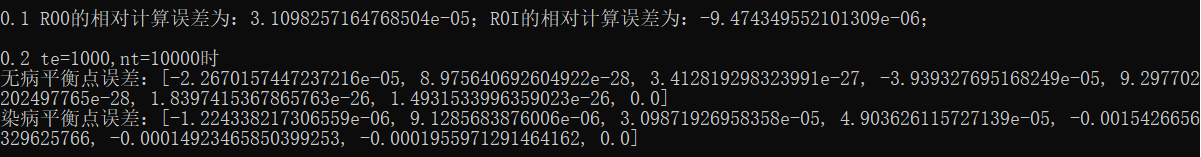
\includegraphics[width=\linewidth]{0.0.png}
    \caption{数值模拟方法准确性测试}
    \label{fig.0.0}
\end{figure}
从图\ref{fig.0.0}可以发现计算结果的相对误差均在0.1\%以下,考虑到计算时取的时间($t_{e}$)为1000未达最终平衡,所以$t_{e}=1000,n_{t}=10000$条件下的准确性基本可以接受。

\subsubsection{精确度验证}
通过递推方法数值模拟求解微分方程组的误差主要来源于时间微分$\delta t$,理论上$\delta t$越小最终的递推结果约精确。但实际计算过程中$\delta t$越小计算耗时也越多,在精度提高不大的情况下一味地减小$\delta t$得不偿失。
\begin{figure}[H]
    \centering
    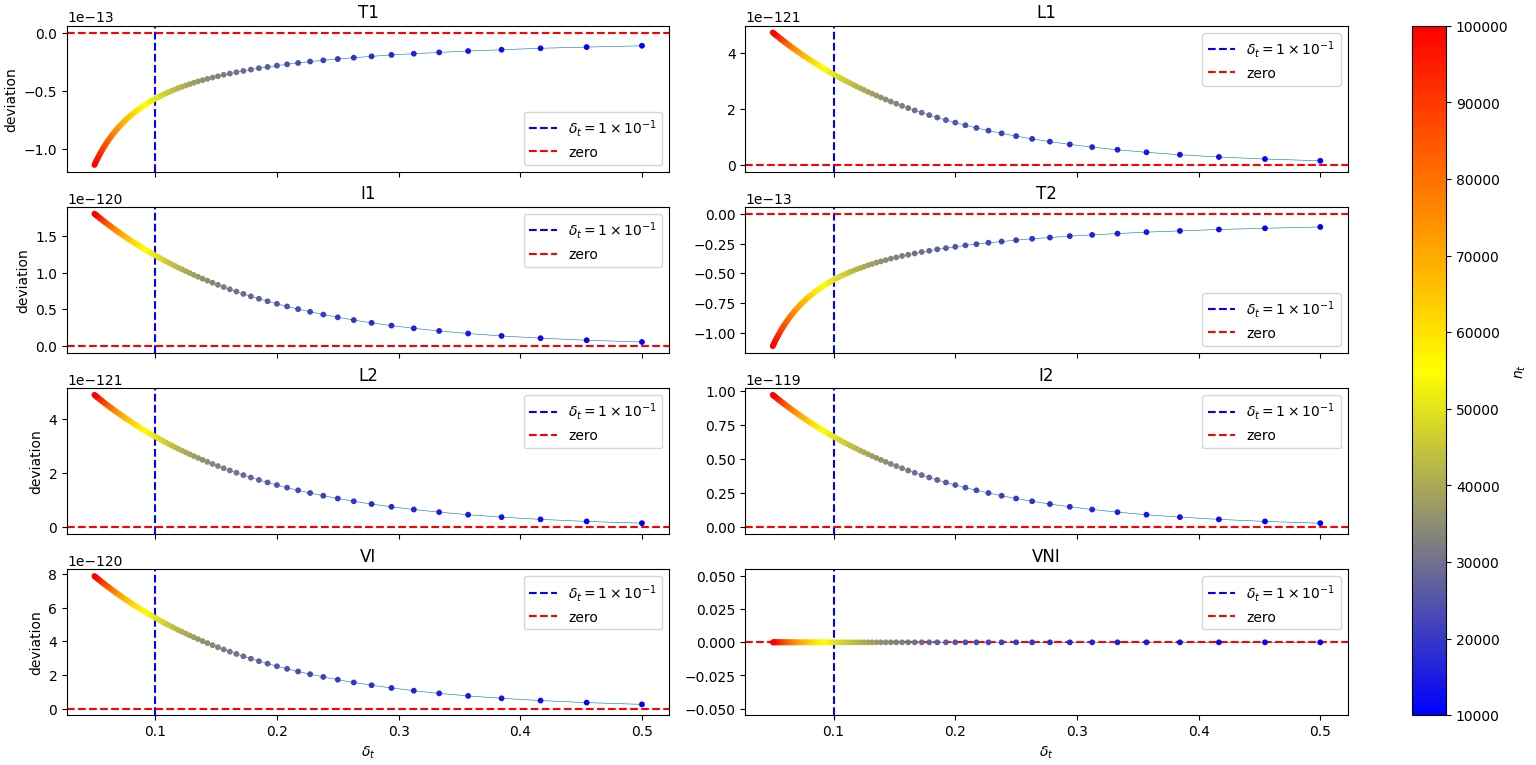
\includegraphics[width=\linewidth]{0.1.png}
    \caption{终态误差与$\delta t$的关系}
    \label{fig.0.1}
\end{figure}
从图\ref{fig.0.1}中可以发现取$\delta t=0.1$时计算结果的误差已经均在\num{e-12}以下及时再减小$\delta t$提高精度意义也不大,所以在后续的计算中均采用$t_{e}=1000,n_{t}=10000$,即$\delta t=0.1$。

\subsection{计算绘图所用数据}
\subsubsection{特定params的计算}
定义函数params\_R0()计算给定条件下的params用于进行感染模型的数值模拟。函数参数:
\begin{enumerate}
    \item n:指定要计算多少组params,即进行多少次数值模拟。
    \item nature:若为False即$\beta_{1},\beta_{2}$服从均匀分布,并且由$R_{0}$(形参:R0\_min=0,R0\_max=2)来筛选;若为True即$\beta_{1},\beta_{2}$服从正态分布,需给出其对应分布参数(形参:b1m=6e-4,b1d=2e-4,b2m=9e-2,b2d=3e-2)。
    \item drug:若为False即不施加药物,$\varepsilon _{RT},\varepsilon _{PI}$均为0;若为True即视药效亦服从正态分布,需要传入相关参数(eRTm=0.25,eRTd=0,ePIm=0.25,ePId=0)。
\end{enumerate}
最终返回一个含五个分别储存可变参数($\beta_{1},\beta_{2},\varepsilon _{RT},\varepsilon _{PI},R_{0}$)的数组的列表,且各数组均根据$R_{0}$按从小到大排序。
\begin{lstlisting}[label={lst.5}, caption={特定params的计算}]
    def params_R0(n=100,nature:bool=False,R0_min=0,R0_max=2,b1m=6e-4,b1d=2e-4,b2m=9e-2,b2d=3e-2,drug:bool=False,eRTm=0.25,eRTd=0,ePIm=0.25,ePId=0):
    if (nature!=True and nature!=False) or (drug!=True and drug!=False):
        print('...')
    else:
        k,R0_pass=0,False
        b1, b2, eRT, ePI, R0=[],[],[],[],[]
        while k<n:
            if nature:
                b1_random, b2_random = np.random.normal(b1m,b1d), np.random.normal(b2m,b2d)
                R0_pass=True
            else:
                b1_random, b2_random = random.uniform(1e-5,0.5), random.uniform(1e-5,0.5)
            if drug:
                eRT_random, ePI_random = np.random.normal(eRTm,eRTd), np.random.normal(ePIm,ePId)
            else:
                eRT_random, ePI_random = 0,0
            R0_random=cell.R0([b1_random,b2_random,0,0,0,0])
            if (R0_min<=R0_random<=R0_max or R0_pass) and b1_random>=0 and b2_random>=0:
               k+=1
               b1.append(b1_random)
               b2.append(b2_random)
               eRT.append(eRT_random)
               ePI.append(ePI_random)
               R0.append(cell.R0([b1_random,b2_random,eRT_random,eRT_random,ePI_random,ePI_random]))
        sorted_index=np.argsort(R0)
        return [(np.array(b1))[sorted_index],(np.array(b2))[sorted_index],(np.array(eRT))[sorted_index],(np.array(ePI))[sorted_index],(np.array(R0))[sorted_index]]
\end{lstlisting}

\subsubsection{不同条件下感染过程的计算}
定义函数$cells\_processes\_params()$计算不同params(可变参数)情况下的感染过程。函数参数:
\begin{enumerate}
    \item $params\_variable$:一个含五个分别储存可变参数($\beta_{1},\beta_{2},\varepsilon _{RT},\varepsilon _{PI},R_{0}$)的数组的列表,且各数组均根据$R_{0}$按从小到大排序。一般就是函数params\_R0的返回值。
    \item cell0:一个包含了八种细胞及病毒初始值的列表。
    \item order:若为'all'则返回不同感染全过程数据组成的列表;若为'final'则仅返回各感染过程终态细胞及病毒浓度组成的列表,同时会将params和终态数据写入'filename.xlsx'的'sheet\_name'(booksheet)中,得到'.xlsx'文件中各列储存数据为:A:$\beta_{1}$; B:$\beta_{2}$; C:$\varepsilon _{RT}$; D:$\varepsilon _{PI}$; E:$R_{0}$; F:$T_{1}$; G:$L_{1}$; H:$I_{1}$; I:$T_{2}$; J:$L_{2}$; K:$I_{2}$; L:$V_{I}$; M:$V_{NI}$;'。
\end{enumerate}
\begin{lstlisting}
    def cells_processes_params(params_variable=None,cell0=[1000,0,0,4,0,0,0,0],order:'all' or 'final'='final',filename=None,sheet_name=str(0)):
\end{lstlisting}

\subsubsection{从'.xlsx'文件中读取数据}
定义函数get\_from\_xlsx()从先前生成的'.xlsx'文件中读取数据,并且再次按照$R_{0}$的值从小到大进行排序,最后返回返回两个二维数组:
\begin{enumerate}
    \item sorted\_data[:5]:含$\beta_{1},\beta_{2},\varepsilon _{RT},\varepsilon _{PI}$值的五个一维数组。
    \item sorted\_data[5:]:含$T_{1},L_{1},I_{1},T_{2},L_{2},I_{2},V_{I},V_{NI}$终态值的八个一维数组。
\end{enumerate}
\begin{lstlisting}[label={lst.6}, caption={读取数据并根据$R_{0}$排序}]
    def get_from_xlsx(filename='cells_processes_params',sheet_name=str(0)):
        df=pd.read_excel(filename+'.xlsx',sheet_name=sheet_name,header=None)
        data=(df.values).T
        sorted_index=np.argsort(data[4])
        sorted_data=data[:,sorted_index]
        print(f'...')
        return sorted_data[:5],sorted_data[5:]
\end{lstlisting}

\subsection{可视化数值模拟过程及终态}
\subsubsection{HIV感染感染过程中各细胞及病毒浓度变化图}
定义函数fig\_cells\_processing\_cell0s(),通过二维列表cell0s(由列表$[T_{1},L_{1},I_{1},T_{2},L_{2},I_{2},V_{I},V_{NI}]$组成)传入不同的初始状态,再通过列表params传入给定的可变参数($\beta_{1},\beta_{2},\varepsilon _{1RT},\varepsilon _{2RT},\varepsilon _{1PI},\varepsilon _{2PI}$),以此绘制不同初始状态在相同可变参数条件下的感染过程。

而定义函数fig\_cells\_processing\_paramses(),通过列表cell0传入一给定初始状态,再通过二维列表paramses(由列表$[\beta_{1},\beta_{2},\varepsilon _{1RT},\varepsilon _{2RT},\varepsilon _{1PI},\varepsilon _{2PI}]$组成)传入不同可变参数,即可绘制相同初值在不同可变参数下的感染过程。
\begin{lstlisting}
    def fig_cells_processing_cell0s(cell0s=[[1000,0,0,4,0,0,0,0]],params=[0.0001,0.015,0,0,0,0],te=1000,nt=10000):
    def fig_cells_processing_paramses(cell0=[1000,0,0,4,0,0,0,0],paramses=[[0.0001,0.015,0,0,0,0]],te=1000,nt=10000):
\end{lstlisting}

\subsubsection{感染终态与$R_{0}$关系图}
定义函数fig\_final\_R0(),通过字典params\_variables和cells\_finals分别传入多对二维数组params\_variable和列表cell\_final(细胞及病毒终态数据)\footnote{从函数cells\_processes\_params()生成的'.xlsx'文件中读取。},以绘制不同$R_{0}$条件下不同初始状态对应的感染终态图。
\begin{lstlisting}
    def fig_final_R0(params_variables=None,cells_finals=None):
\end{lstlisting}

\subsubsection{$R_{0}$与$\beta_{1},\beta_{2}$关系图}
定义函数fig\_R0\_b1\_b2(),通过列表params\_variable传入params以绘制$R_{0}$与$\beta_{1},\beta_{2}$关系图。
\begin{lstlisting}
    def fig_R0_b1_b2(params_variable=None):
\end{lstlisting}

\subsubsection{感染终态与$\beta_{1},\beta_{2}$关系图}
定义函数fig\_final\_b1\_b2(),传入二维数组params\_variable和cells\_final\footnote{从函数cells\_processes\_params()生成的'.xlsx'文件中读取。}绘制感染终态与$\beta_{1},\beta_{2}$关系图。
\begin{lstlisting}
    def fig_final_b1_b2(params_variable=None,cells_final=None):
\end{lstlisting}

\subsubsection{$R_{0}$与$\varepsilon _{RT},\varepsilon _{PI}$关系图}
定义函数fig\_drug\_effect(),传入参数$\beta_{1},\beta_{2}$后即可绘制$R_{0}$随$\varepsilon _{RT},\varepsilon _{PI}$变化图。
\begin{lstlisting}
    def fig_drug_effect(b1=0.0006,b2=0.015):
\end{lstlisting}

\subsubsection{有无药物时治愈率对比图}
定义函数fig\_compare\_healing\_b1\_b2(),函数参数:
\begin{enumerate}
    \item params\_variable\_nodrug :无药时的可变参数及$R_{0}$。
    \item cells\_final\_nodrug :无药时的感染终态。
    \item params\_variable\_drug :有药时的可变参数及$R_{0}$。
    \item cells\_final\_drug :有药时的感染终态。
    \item tol:误差标准,只要两种免疫细胞$T_{1},T_{2}$均恢复到自身正常水平\footnote{无病平衡点:$T_{1}=1000,T_{2}=4$。}的(1-tol),即可认为治愈。
\end{enumerate}
基于上述数据即可绘制有无药物时的治愈率对比图。
\begin{lstlisting}
    def fig_compare_healing_b1_b2(params_variable_nodrug=None,cells_final_nodrug=None,params_variable_drug=None,cells_final_drug=None,tol=1e-2):
\end{lstlisting}

\subsubsection{自然条件下治愈率与药效关系图}
定义函数fig\_rate\_drug\_nature(),绘制自然状态($\beta_{1},\beta_{2}$均呈正态分布)下,施加单种药物和两种药物联合治疗的治愈率与药效关系图。
\begin{lstlisting}
    def fig_rate_drug_nature():
\end{lstlisting}

\section{创新性}
\subsection{利用类来运算并储存一阶线性微分方程组}
观察“两种靶细胞的HIV感染模型”(一阶线性微分方程组),可以发现每个微分方程对应变量的一阶微分不仅与自身有关还与其他方程的变量也有关,这使得求解解析解十分困难。由于无法得知各一阶微分的解析式,故只有采用递推公式$$cell[i+1]=cell[i]+\dot{cell}[i]\cdot \delta t$$进行近似计算,又由于各变量一阶微分均由多个变量共同决定,不便于单独计算某一变量的变化过程,所以使用递推的方法,在每轮递推循环中利用上一轮求得的变量值求出本轮所有的变量值,如此进行直到达预期的递推次数。

由于方程组中参数多且相同,各变量的递推公式形式相同,故创建父类Cell(见代码\ref{lst.1}),在构造方法中变设定好恒定参数,同时创建数组self. cell\_process= np.zeros(int(nt +1))用来存储计算过程中的变量变化,还创建类方法process()即递推公式。各子类(代表八种细胞及病毒,见代码\ref{lst.2})继承了Cell的恒定参数,储存数组和递推公式的同时加入了各自的初值$cell_{0}$,并且根据自身的微分方程创建替代父类的dnumber()。

最后利用函数all\_cells\_processes(),一次同时实例化八个子类,依靠初始值$cell_{0}s$进行$n_{t}$轮递推,每轮均计算出八种变量的值并且存于相应对象的数组中,递推完成后即实现了一次HIV感染模型的数值模拟。

\subsection{利用'.xlsx'文件存储而非实时计算绘图数据}
在绘制感染终态与不同可变参数(params)的关系图中需要计算多种params条件下的感染过程,即进行多次数值模拟计算感染过程才能绘制出一张图。尤其是计算治愈率时,对于每一种药效组合均需计算至少100次感染过程才能统计该组合的治愈率,而若想让治愈率的计算更加精准需计算的感染过程次数更多。单次感染过程的计算量已经在\num{8e4}规模,如果实时计算绘图所需数据耗时耗力,且绘图结束后便舍弃相关数据也十分浪费。故创建函数cells\_processes\_params(),将每次计算的结果储存在'.xlsx'文件中,绘图时再通过函数get\_from\_xlsx()从文件中读取数据,极大节省了绘图时间。同时可以分多次计算后合并得大量数据,充分节省计算资源。
\begin{lstlisting}[label={lst.7}, caption={生成感染终态数据并在'.xlsx'文件中存读}]
    def cells_processes_params(params_variable=None,cell0=[1000,0,0,4,0,0,0,0],order:'all' or 'final'='final',filename=None,sheet_name=str(0)):
    if order!='all' and order!='final':
        print('...')
    else:
        n=len(params_variable[0])
        if order=='final':
            R0_cells_final=[]
            for i in tqdm(range(n),desc=f'cell0:{cell0},cells processing'):
                R0_cells_final.append(all_cells_processes(cell0=cell0,params=[params_variable[0][i],params_variable[1][i],params_variable[2][i],params_variable[2][i],params_variable[3][i],params_variable[3][i]],order='final'))
            cells_final=np.array(R0_cells_final)
            if filename:
                data=np.concatenate((np.array(params_variable).T,cells_final),axis=1)
                try:
                    wb = openpyxl.load_workbook(filename=filename+'.xlsx')
                except FileNotFoundError:
                    wb = openpyxl.Workbook()
                    wb.remove(wb['Sheet'])
                if sheet_name in wb.sheetnames:
                    ws = wb[sheet_name]
                    k=0
                else:
                    ws = wb.create_sheet(sheet_name)
                    k=1
                last_row = ws.max_row-k
                lrow=last_row
                print(f'...')
                for row in data:
                    last_row += 1
                    for column, value in enumerate(row, start=1):
                        ws.cell(row=last_row, column=column, value=value)
                wb.save(filename=filename+'.xlsx')
                print(f'...')
            return cells_final.T
        elif order=='all':
            R0_cells_processes=[]
            for i in tqdm(range(n),desc=f'cell0:{cell0},cells processing'):
                R0_cells_processes.append(all_cells_processes(cell0=cell0,params=[params_variable[0][i],params_variable[1][i],params_variable[2][i],params_variable[2][i],params_variable[3][i],params_variable[3][i]],order='all_noreport'))
            return np.array(R0_cells_processes)

def get_from_xlsx(filename='cells_processes_params',sheet_name=str(0)):
    df=pd.read_excel(filename+'.xlsx',sheet_name=sheet_name,header=None)
    data=(df.values).T
    sorted_index=np.argsort(data[4])
    sorted_data=data[:,sorted_index]
    print(f'...')
    return sorted_data[:5],sorted_data[5:]
\end{lstlisting}

\section{运行方法和参数设置}
\subsection{运行方法}
本程序的主要功能便是对“包含潜伏感染阶段的具有两种靶细胞的HIV感染模型”进行数值模拟并且将结果可视化,考虑到该模型的大量参数已经固定(见表\ref{tab.1}),故在无特殊要求的情况下就根据默认初始值进行数值模拟和绘图,所以运行方法十分简便。
\begin{figure}[H]
    \centering
    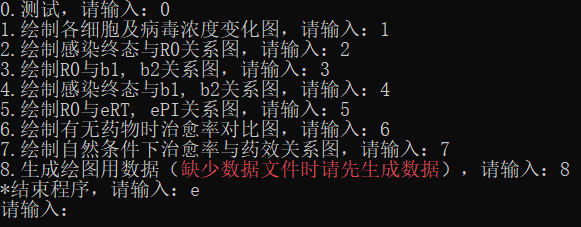
\includegraphics[width=0.6\linewidth]{0.01.png}
    \caption{用户界面输入提示词}
    \label{fig.0.01}
\end{figure}
运行'HIV.py'文件后,根据输入提示词(见图\ref{fig.0.01}),输入相应的字符作为指令即可进行测试、生成数据\footnote{\textcolor{red}{在缺少数据文件时要先进行一次数据生成再绘制图表。}}以及绘制相应图表:
\begin{enumerate}
    \item 绘制各细胞及病毒浓度变化图;
    \item 绘制感染终态与$R_{0}$关系图;
    \item 绘制$R_{0}$与$\beta_{1},\beta_{2}$关系图;
    \item 绘制感染终态与$\beta_{1},\beta_{2}$关系图;
    \item 绘制$R_{0}$与$\varepsilon _{RT},\varepsilon _{PI}$关系图;
    \item 绘制有无药物时治愈率对比图;
    \item 绘制自然条件下治愈率与药效关系图;
\end{enumerate}

\subsection{参数设置}
生物体是一个高度动态且个体差异较大的系统,一个模型无法同时适配所有的情况,所以在面对特定群体或根据最新的研究结果有时候也需要更改数值模拟的参数,这里以默认值为例,说明如何设置参数,并展示相应绘图结果。
\subsubsection{绘制各细胞及病毒浓度变化图}
\paragraph{不给药时感染过程}:四种初始状态($cell_{0}s=[[900,2,7,2,0.15,0.5,18,0],$\\$[700,1.5,5,1.5,0.0005,0.0005,15,0],[500,1,3,1,0.001,0.001,12,0],[300,0.5,1.5,0.5,0.1,0.3,8,0]]$)分别在两种可变参数params([0.0001,0.015,0,0,0,0],[0.0006,0.001,0,0,0,0])条件下的感染过程,模拟时间($t_{e}$)分别为800day,500day。
    \begin{lstlisting}
    cell0s=np.array([[900,2,7,2,0.15,0.5,18,0],[700,1.5,5,1.5,0.0005,0.0005,15,0],
    [500,1,3,1,0.001,0.001,12,0],[300,0.5,1.5,0.5,0.1,0.3,8,0]])
    fig_cells_processing_cell0s(cell0s=cell0s,params=[0.0001,0.015,0,0,0,0],te=800,nt=16000)
    fig_cells_processing_cell0s(cell0s=cell0s,params=[0.0006,0.001,0,0,0,0],te=500,nt=10000)
\end{lstlisting}
    \begin{figure}[H]
        \centering
        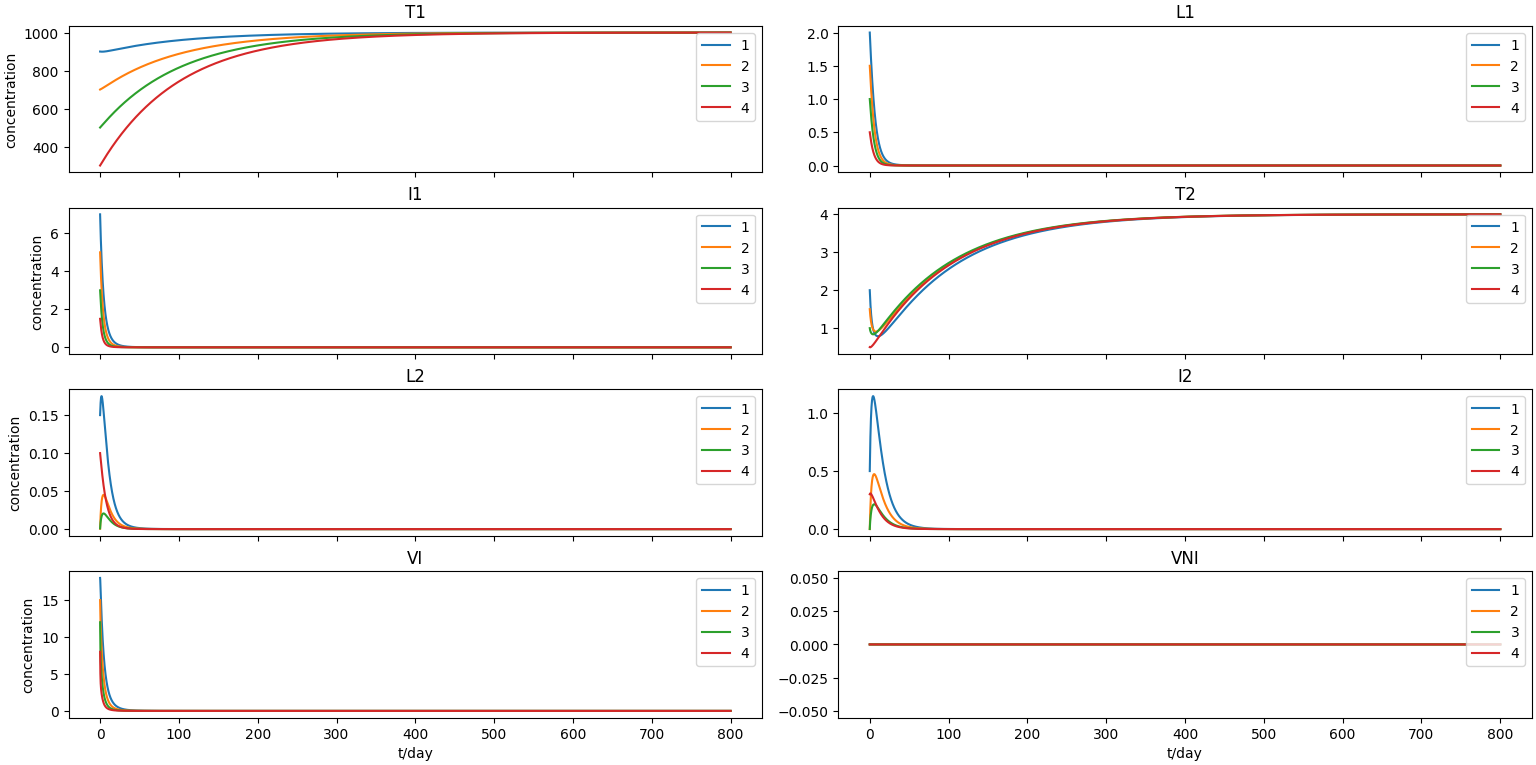
\includegraphics[width=\linewidth]{1.1.png}
        \caption{params=[0.0001,0.015,0,0,0,0]条件下感染过程}
        \label{fig.1.1}
    \end{figure}
    \begin{figure}[H]
        \centering
        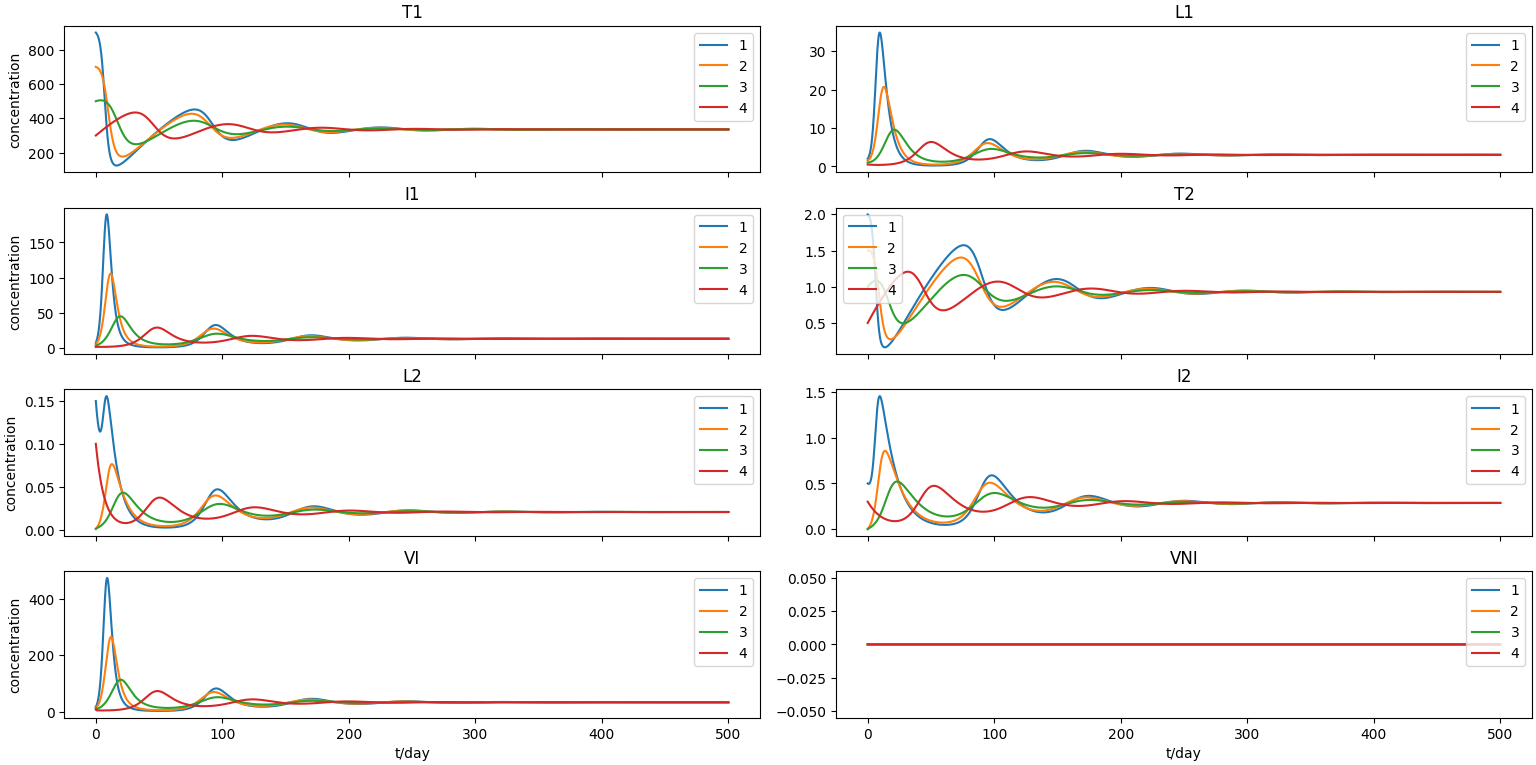
\includegraphics[width=0.95\linewidth]{1.2.png}
        \caption{params=[0.0006,0.001,0,0,0,0]条件下感染过程}
        \label{fig.1.2}
    \end{figure}

    \paragraph{给药时感染过程}:初始状态$cell_{0}=[500,1,3,1,0.001,0.001,12,0]$分别在四种可变参数\\params\_drug=[[0.0006,0.001,0.13,0.13,0.23,0.23],[0.0006,0.001,0.23,0.23,0.33,0.33],[0.0006,0.001,0.33,0.33,0.43,0.43]\\,[0.0006,0.001,0.43,0.43,0.53,0.53]]条件下的感染过程,模拟时间($t_{e}$)分别为1500day。
    \begin{lstlisting}
    params_drug=[[0.0006,0.001,0.13,0.13,0.23,0.23],[0.0006,0.001,0.23,0.23,0.33,0.33],
    [0.0006,0.001,0.33,0.33,0.43,0.43],[0.0006,0.001,0.43,0.43,0.53,0.53]]
    fig_cells_processing_paramses(cell0=[500,1,3,1,0.001,0.001,12,0],paramses=params_drug,te=1500,nt=30000)
\end{lstlisting}
    \begin{figure}[H]
        \centering
        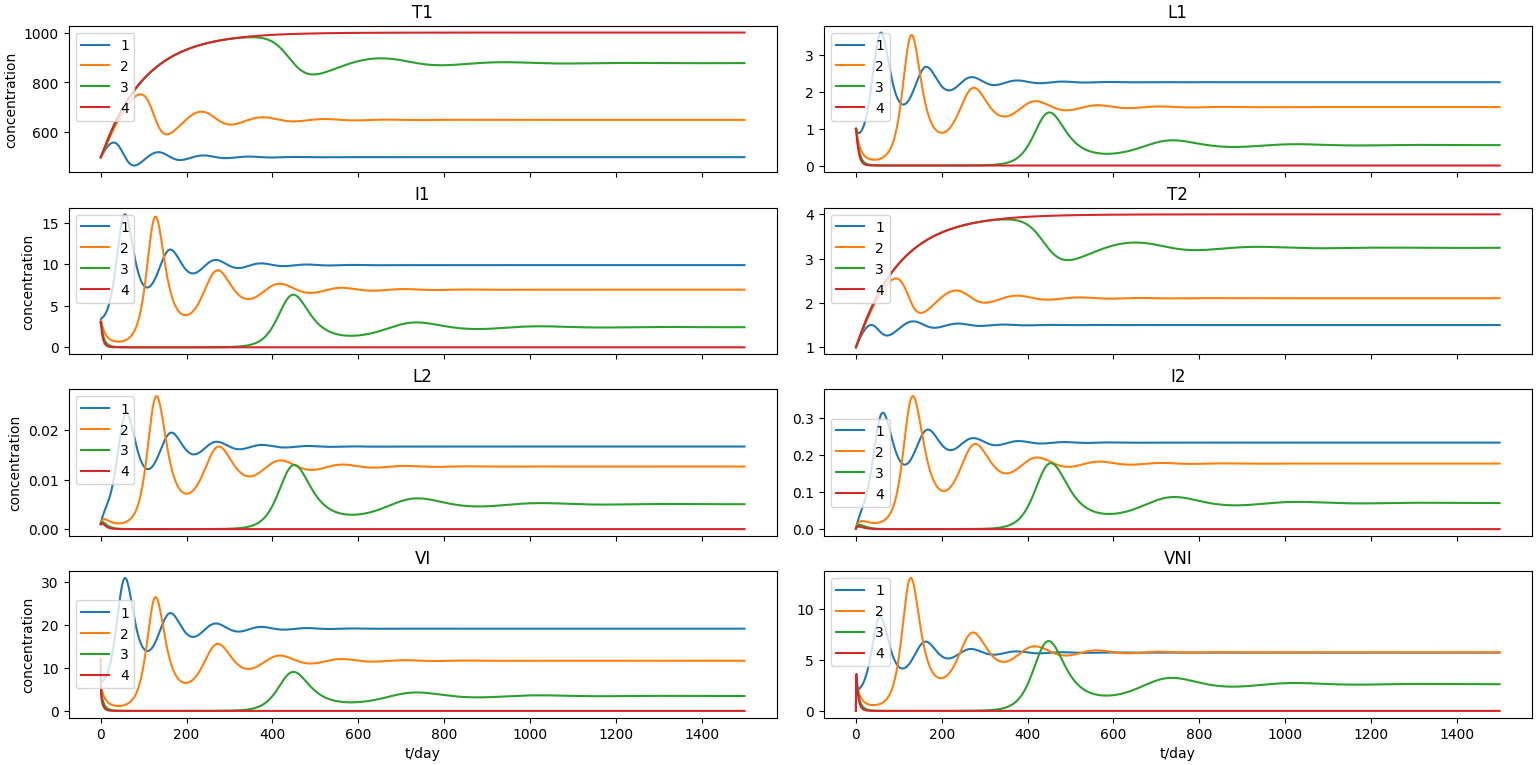
\includegraphics[width=0.95\linewidth]{1.3.png}
        \caption{$cell_{0}=[500,1,3,1,0.001,0.001,12,0]$在给药条件下的感染过程}
        \label{fig.1.3}
    \end{figure}

    \subsubsection{绘制感染终态与$R_{0}$关系图}
    通过函数params\_R0()生成n(100)组可变参数params,且nature=False表明$\beta_{1},\beta_{2}$服从均匀分布($R_{0,min}=0,R_{0,max}=2$),drug=False则表示$\varepsilon _{RT},\varepsilon _{PI}$均为零。

    再利用函数cells\_processes\_params()根据上一步生成的params组,分别对四种初始状态($cell_{0}s$)进行数值模拟,并将params和感染终态存入filename='data\_final\_R0'的'.xlsx'文件中。最后绘图时从文件中读取params和cells\_finals绘制图表。
    \begin{lstlisting}
    params_variable=params_R0(n=100,nature=False,R0_min=0,R0_max=2,drug=False)
    for i,item in enumerate(cell0s):
        params_variables[i],cells_finals[i]=cells_processes_params(params_variable=params_variable,cell0=item,order='final',filename='data_final_R0',sheet_name=str(i))
    for i,item in enumerate(cell0s):
        params_variables[i],cells_finals[i]=get_from_xlsx(filename='data_final_R0',sheet_name=str(i))
    fig_final_R0(params_variables=params_variables,cells_finals=cells_finals)
    fig_final_R0(params_variables=params_variables,cells_finals=[cells_finals[2]])
\end{lstlisting}
    \begin{figure}[H]
        \centering
        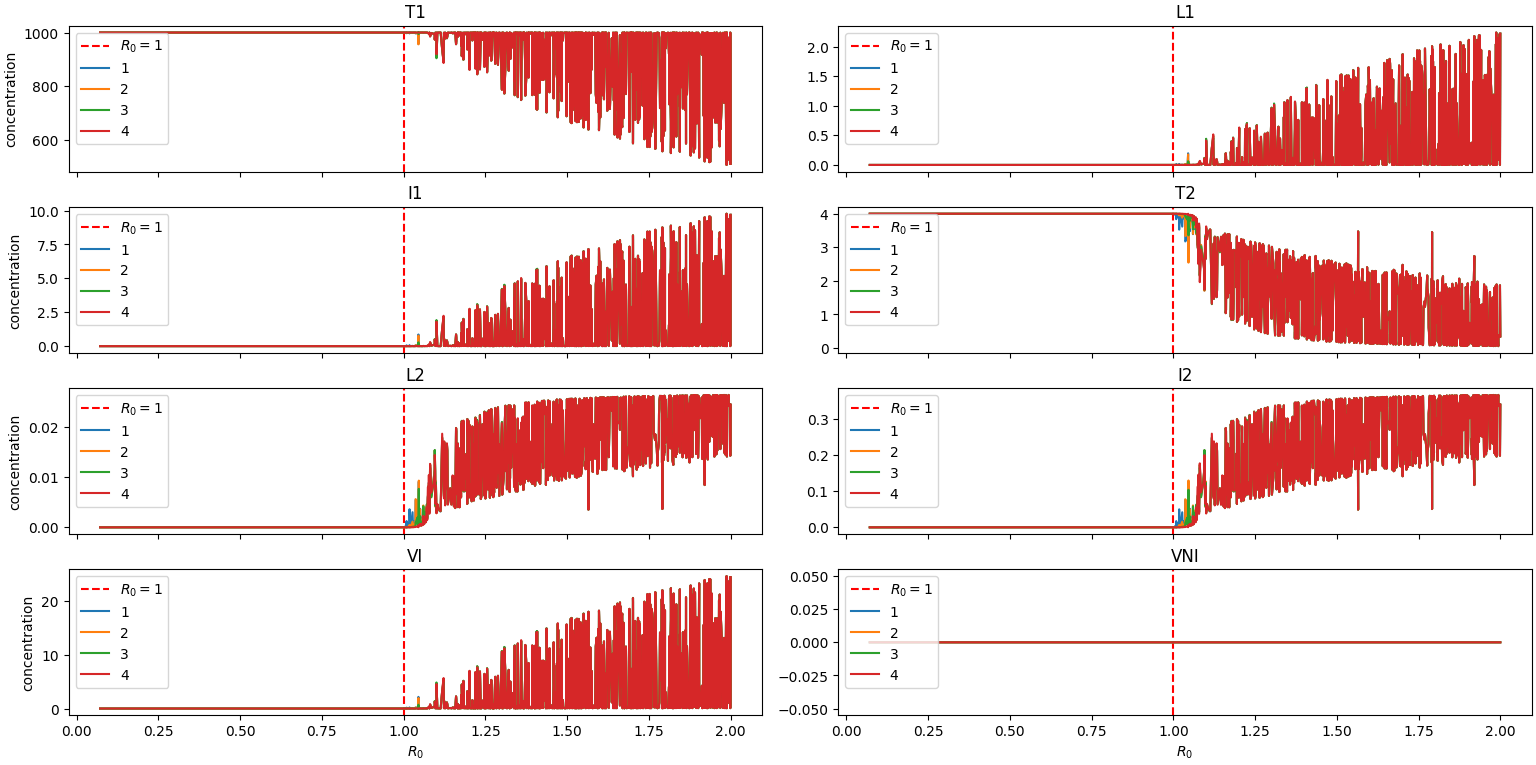
\includegraphics[width=0.95\linewidth]{2.1.png}
        \caption{四种初始状态的感染终态随$R_{0}$变化图}
        \label{fig.2.1}
    \end{figure}
    \begin{figure}[H]
        \centering
        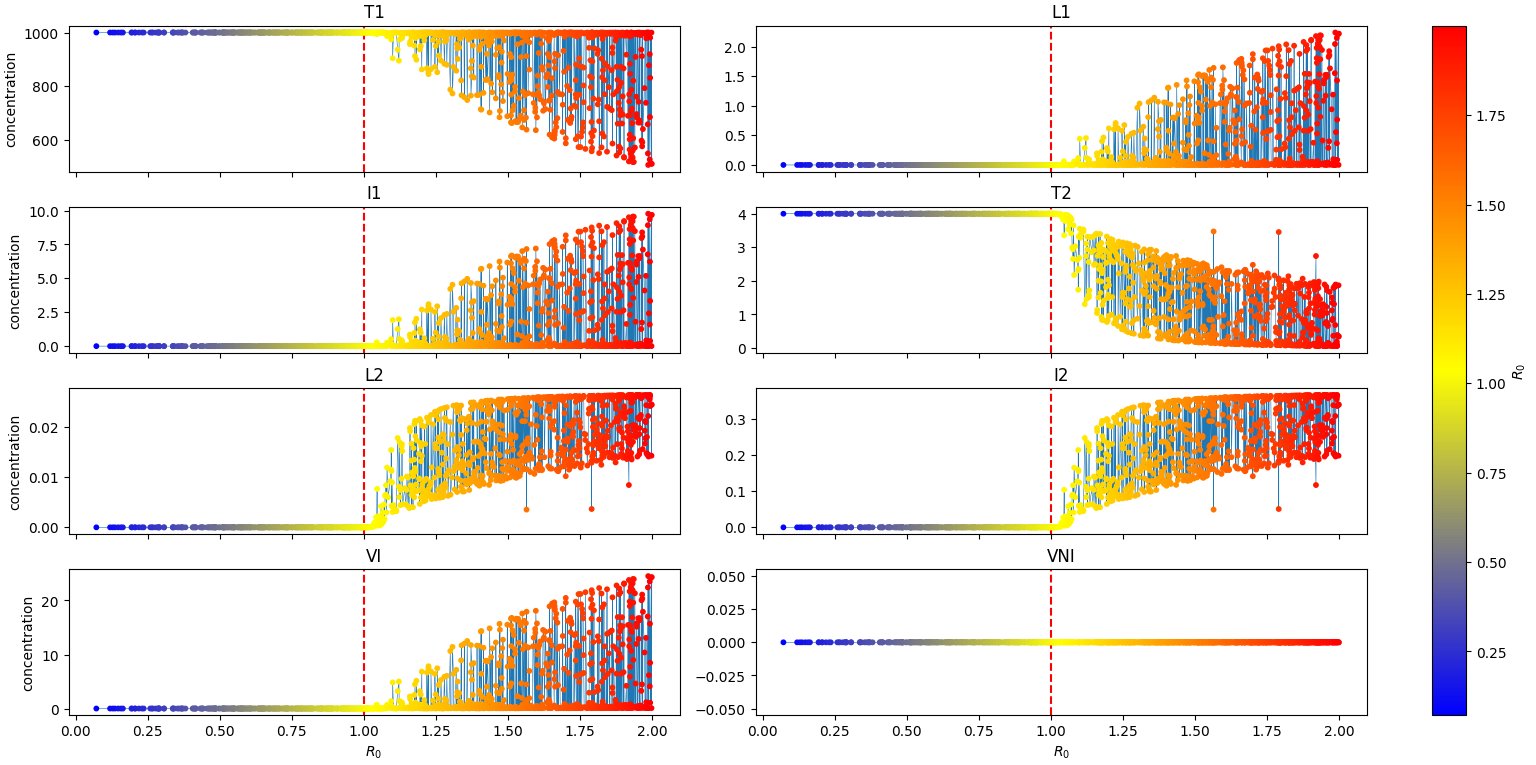
\includegraphics[width=0.95\linewidth]{2.2.png}
        \caption{$cell_{0}=[500,1,3,1,0.001,0.001,12,0]$的感染终态随$R_{0}$变化图}
        \label{fig.2.2}
    \end{figure}

    \subsubsection{绘制$R_{0}$与$\beta_{1},\beta_{2}$关系图}
    利用函数params\_R0()生成的params组还可以用来绘制$R_{0}$与$\beta_{1},\beta_{2}$关系图。理想条件下的参数设置同上;而自然条件即nature=True时表明感染率$\beta_{1},\beta_{2}$分别服从正态分布$(\beta_{1}\sim N(\num{6e-4},(\num{2e-4})^{2}),\beta_{2}\sim N(\num{9e-2},(\num{3e-2})^{2}))$\cite{7}。根据得到的params组即可绘制$R_{0}$与$\beta_{1},\beta_{2}$关系图。
    \begin{lstlisting}
    params_variable=params_R0(n=5000,nature=False,R0_min=0,R0_max=2,drug=False)
    fig_R0_b1_b2(params_variable)
    params_variable=params_R0(n=5000,nature=True,b1m=6e-4,b1d=2e-4,b2m=9e-2,b2d=3e-2,drug=False)
    fig_R0_b1_b2(params_variable)
\end{lstlisting}
    \begin{figure}[H]
        \centering
        \begin{subfigure}[b]{0.48\linewidth}
            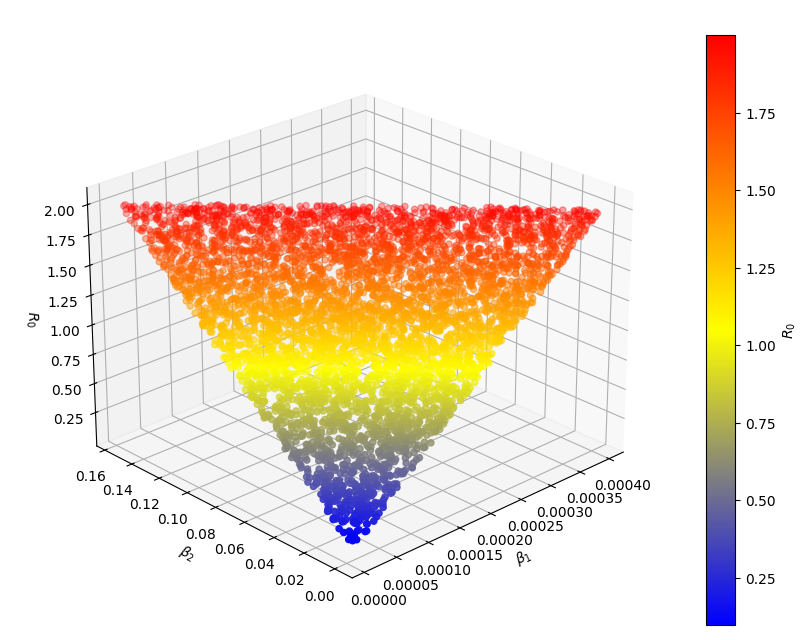
\includegraphics[width=\linewidth]{3.1.1.png}
            \caption{理想条件$R_{0}$与$\beta_{1},\beta_{2}$关系图(3D)}
            \label{fig.3.1.1}
        \end{subfigure}
        \begin{subfigure}[b]{0.48\linewidth}
            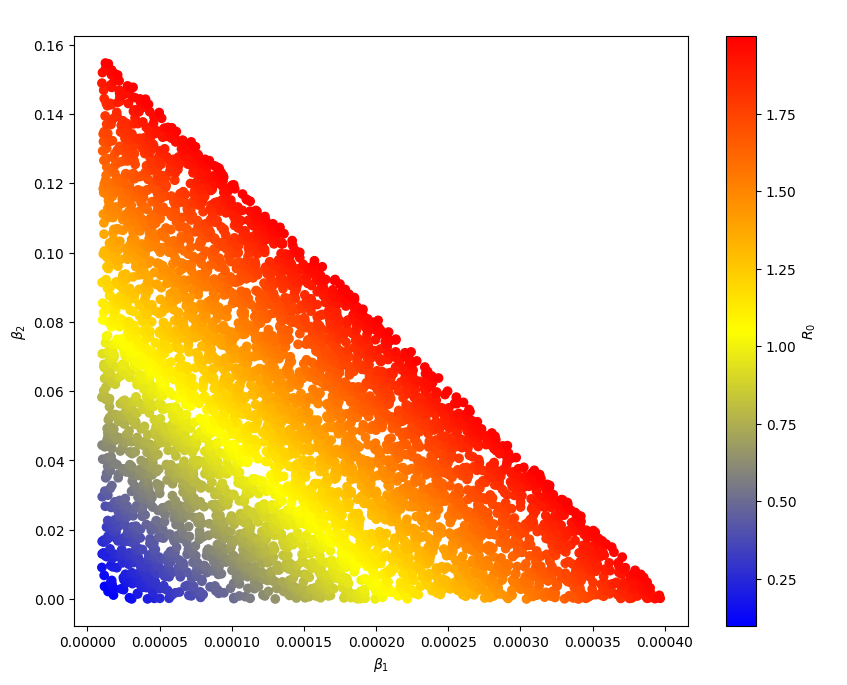
\includegraphics[width=\linewidth]{3.1.2.png}
            \caption{理想条件$R_{0}$与$\beta_{1},\beta_{2}$关系图(2D)}
            \label{fig.3.1.2}
        \end{subfigure}
        \caption{理想条件$R_{0}$与$\beta_{1},\beta_{2}$关系图}
        \label{fig.3.1.1-2}
    \end{figure}
    \begin{figure}[H]
        \centering
        \begin{subfigure}[b]{0.49\linewidth}
            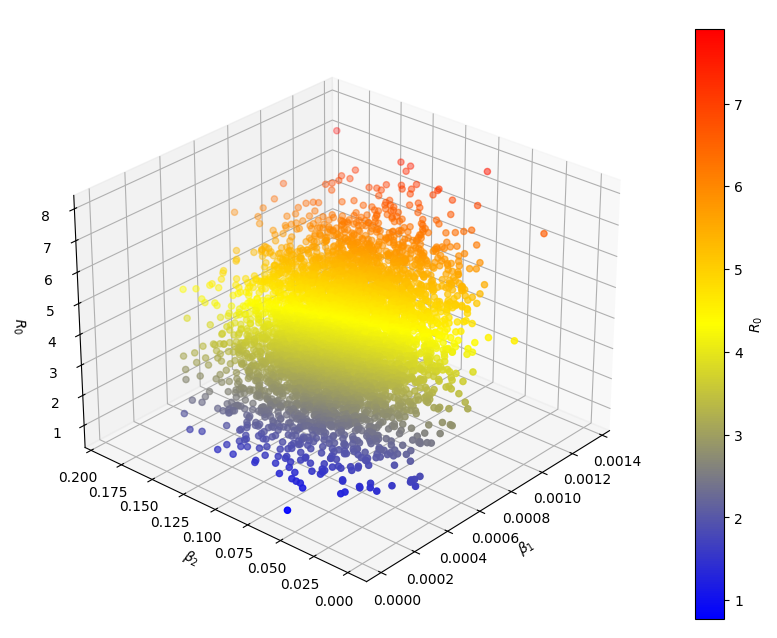
\includegraphics[width=\linewidth]{3.2.1.png}
            \caption{自然条件$R_{0}$与$\beta_{1},\beta_{2}$关系图(3D)}
            \label{fig.3.2.1}
        \end{subfigure}
        \begin{subfigure}[b]{0.49\linewidth}
            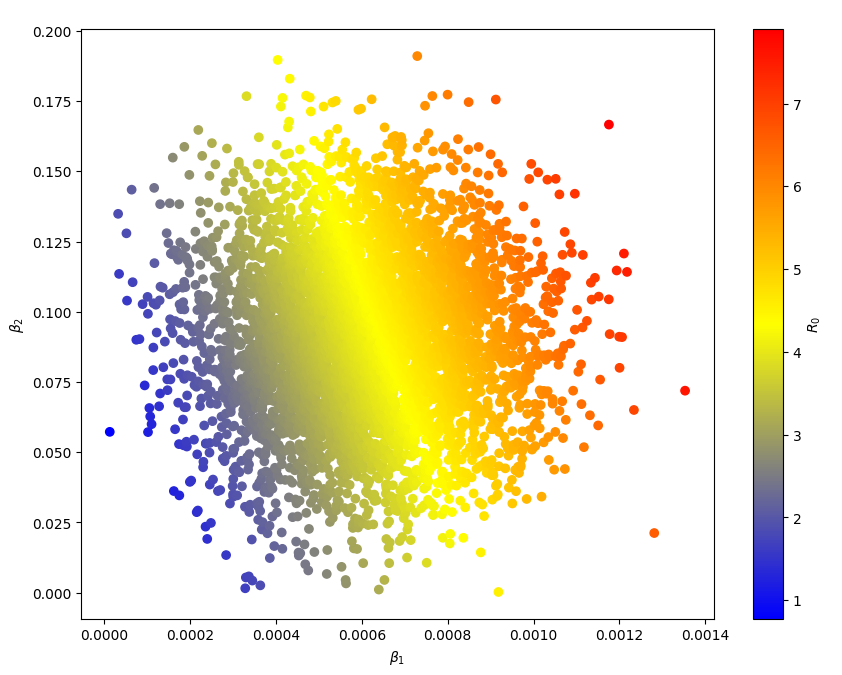
\includegraphics[width=\linewidth]{3.2.2.png}
            \caption{自然条件$R_{0}$与$\beta_{1},\beta_{2}$关系图(2D)}
            \label{fig.3.2.2}
        \end{subfigure}
        \caption{自然条件$R_{0}$与$\beta_{1},\beta_{2}$关系图}
        \label{fig.3.2.1-2}
    \end{figure}

    \subsubsection{绘制感染终态与$\beta_{1},\beta_{2}$关系图}
    将上述的理想条件和自然条件下算得的params组和相应的cells\_final组分别传入函数cells\_processes\_params()即可分别绘制两种条件下的感染终态与$\beta_{1},\beta_{2}$关系图。
    \begin{lstlisting}
    params_variable=params_R0(R0_min=0,R0_max=2,n=50,nature=False,drug=False)
    cells_final=cells_processes_params(params_variable=params_variable,cell0=[500,1,3,1,0.001,0.001,12,0],order='final')
    fig_final_b1_b2(params_variable=params_variable,cells_final=cells_final)
    params_variable=params_R0(n=100,nature=True,b1m=6e-4,b1d=2e-4,b2m=9e-2,b2d=3e-2,drug=False)
    cells_final=cells_processes_params(params_variable=params_variable,cell0=[500,1,3,1,0.001,0.001,12,0],order='final')
    fig_final_b1_b2(params_variable=params_variable,cells_final=cells_final)
\end{lstlisting}
    \begin{figure}[H]
        \centering
        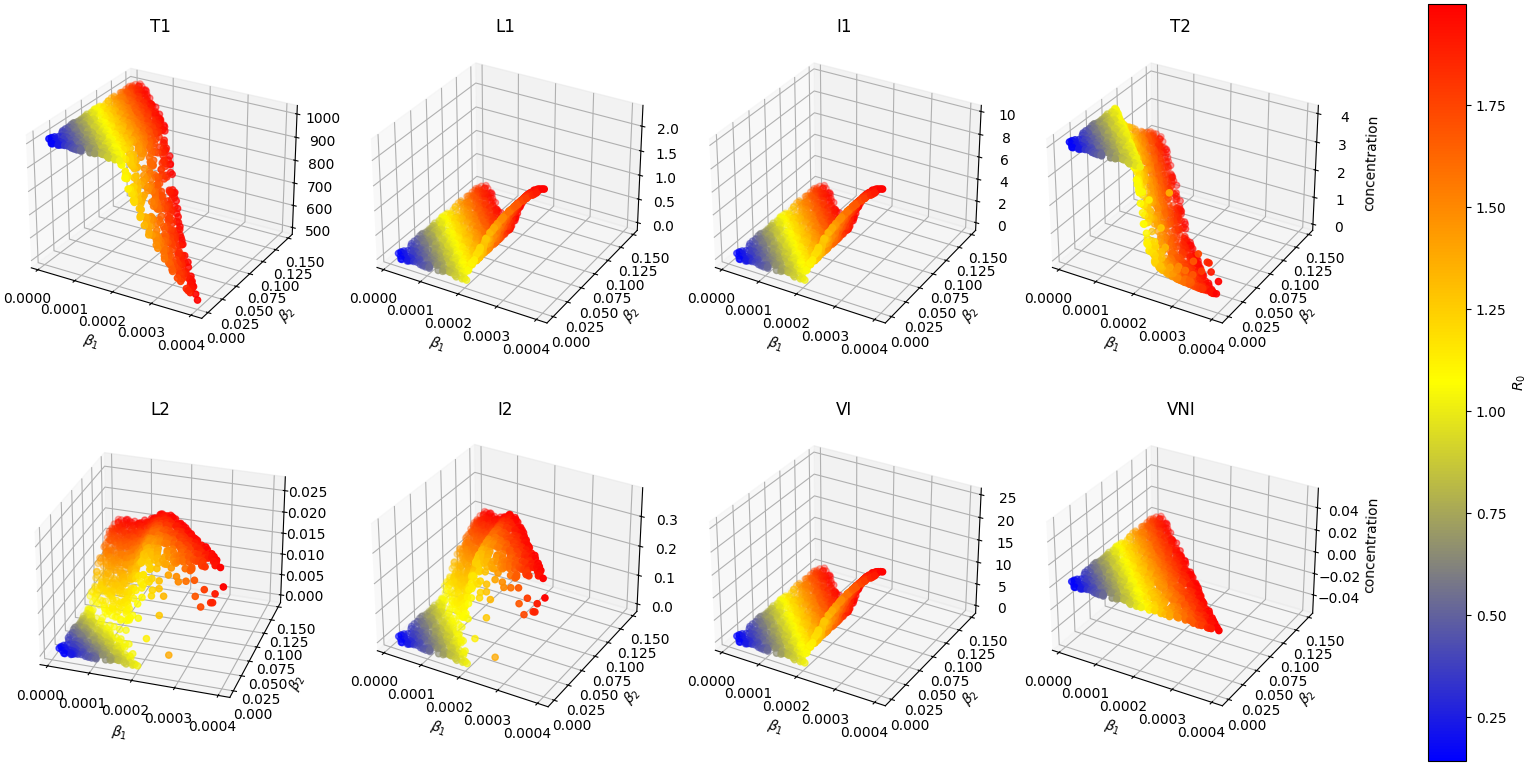
\includegraphics[width=\linewidth]{4.1.png}
        \caption{理想条件感染终态与$\beta_{1},\beta_{2}$关系图}
        \label{fig.4.1}
    \end{figure}
    \begin{figure}[H]
        \centering
        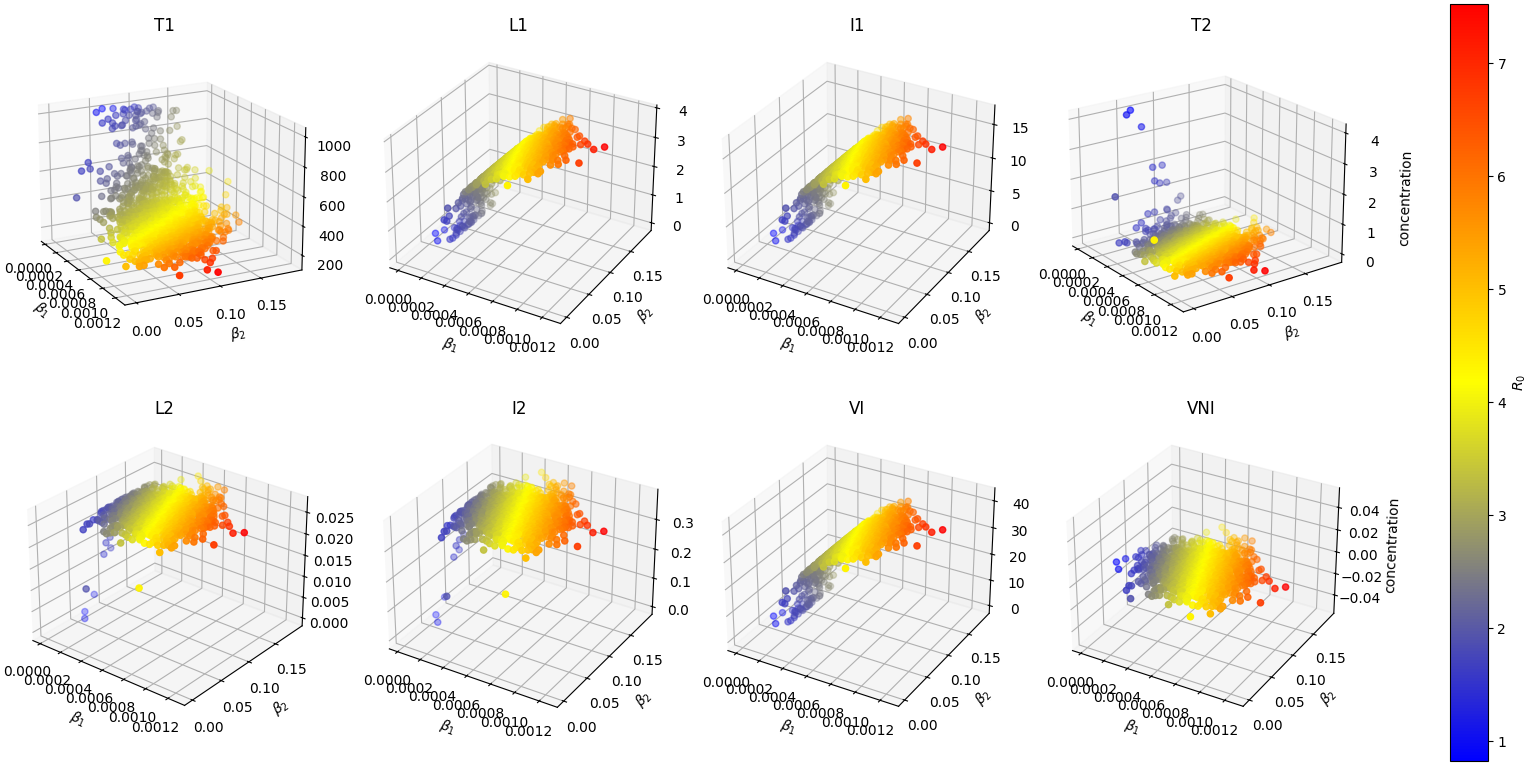
\includegraphics[width=\linewidth]{4.2.png}
        \caption{自然条件感染终态与$\beta_{1},\beta_{2}$关系图}
        \label{fig.4.2}
    \end{figure}

    \subsubsection{绘制$R_{0}$与$\varepsilon _{RT},\varepsilon _{PI}$关系图}
    在设定$\beta_{1}=0.0006,\beta_{2}=0.015$的情况下,绘制$R_{0}$与$\varepsilon _{RT},\varepsilon _{PI}$关系图。
    \begin{lstlisting}
    fig_drug_effect(b1=0.0006,b2=0.015)
\end{lstlisting}
    \begin{figure}[H]
        \centering
        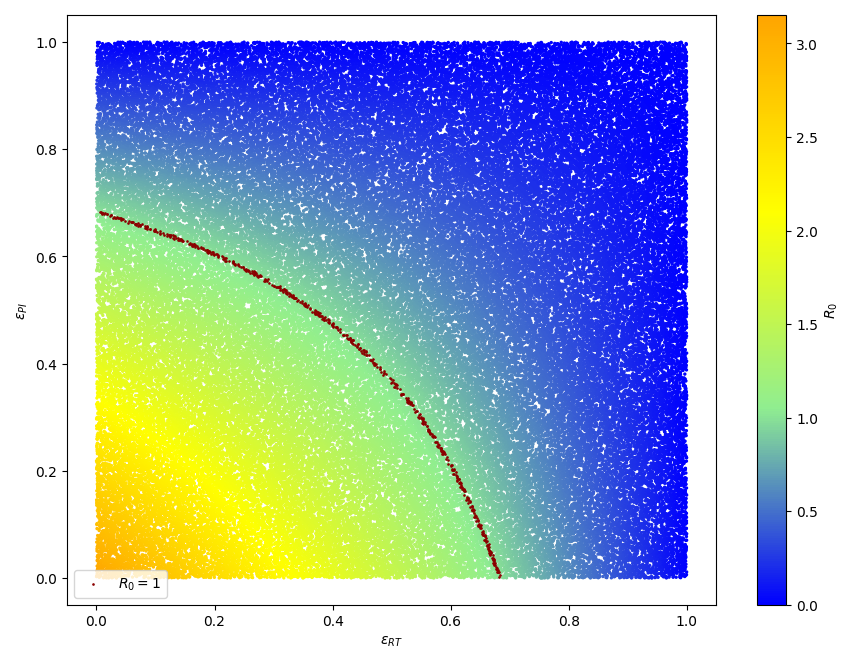
\includegraphics[width=0.8\linewidth]{5.png}
        \caption{$\beta_{1}=0.0006,\beta_{2}=0.015$的情况下$R_{0}$与$\varepsilon _{RT},\varepsilon _{PI}$关系图}
        \label{fig.5}
    \end{figure}

    \subsubsection{绘制有无药物时治愈率对比图}
    \paragraph{理想条件下治愈率对比图}
    生成有药条件下的params组时,drug=True,eRTm=0.25,ePIm=0.25(即$\varepsilon _{RT},\varepsilon _{PI}$的药效均为25\%)。在$cell_{0}=[500,1,3,1,0.001,0.001,12,0]$的情况下计算感染过程得相应感染终态cell\_final组,根据阈值tol(\num{1e-3})来判断是否治愈。
    \begin{lstlisting}
    params_variable_nodrug=params_R0(R0_min=0,R0_max=2,n=20,nature=False,drug=False)
    cells_final_nodrug=cells_processes_params(params_variable=params_variable_nodrug,cell0=[500,1,3,1,0.001,0.001,12,0],order='final')
    params_variable_drug=params_R0(R0_min=0,R0_max=2,n=20,nature=False,drug=True,eRTm=0.25,ePIm=0.25)
    cells_final_drug=cells_processes_params(params_variable=params_variable_drug,cell0=[500,1,3,1,0.001,0.001,12,0],order='final')
    fig_compare_healing_b1_b2(params_variable_nodrug=params_variable_nodrug,cells_final_nodrug=cells_final_nodrug,params_variable_drug=params_variable_drug,cells_final_drug=cells_final_drug,tol=1e-3)
\end{lstlisting}
    \begin{figure}[H]
        \centering
        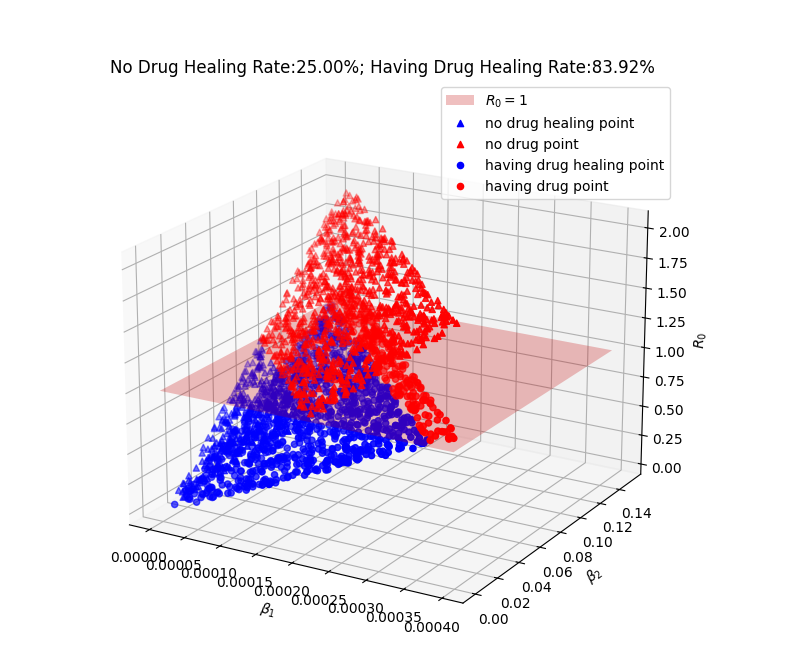
\includegraphics[width=0.8\linewidth]{6.1.1.png}
        \caption{理想条件下治愈率对比图($\varepsilon _{RT}=0.25,\varepsilon _{PI}=0.25$)}
        \label{fig.6.1.1}
    \end{figure}
    \begin{figure}[H]
        \centering
        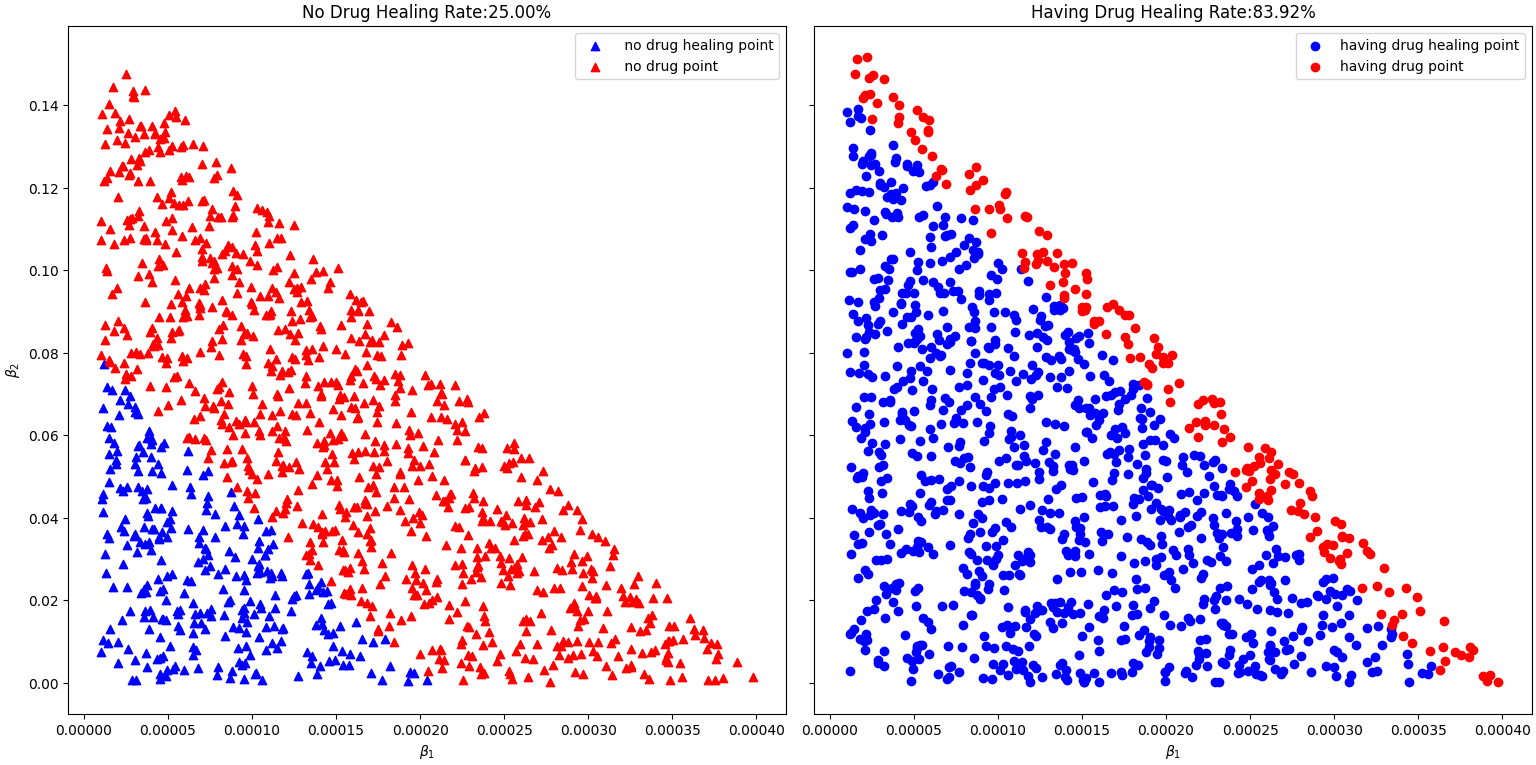
\includegraphics[width=\linewidth]{6.1.2.png}
        \caption{理想条件下治愈率对比图($\varepsilon _{RT}=0.25,\varepsilon _{PI}=0.25$)}
        \label{fig.6.1.2}
    \end{figure}

    \paragraph{自然条件下治愈率对比图}
    nature=True,即感染率$\beta_{1},\beta_{2}$分别服从正态分布$(\beta_{1}\sim N(\num{6e-4},(\num{2e-4})^{2}),\beta_{2}\sim N(\num{9e-2},(\num{3e-2})^{2}))$。生成有药条件下的params组时,drug=True,eRTm=0.5,ePIm=0.5(即$\varepsilon _{RT},\varepsilon _{PI}$的药效均为50\%)。在$cell_{0}=[500,1,3,1,0.001,0.001,12,0]$的情况下计算感染过程得相应感染终态cell\_final组,根据阈值tol(\num{1e-3})来判断是否治愈。
\begin{lstlisting}
    params_variable_nodrug=params_R0(n=50,nature=True,b1m=6e-4,b1d=2e-4,b2m=9e-2,b2d=3e-2,drug=False)
    cells_final_nodrug=cells_processes_params(params_variable=params_variable_nodrug,cell0=[500,1,3,1,0.001,0.001,12,0],order='final')
    params_variable_drug=params_R0(n=50,nature=True,b1m=6e-4,b1d=2e-4,b2m=9e-2,b2d=3e-2,drug=True,eRTm=0.5,ePIm=0.5)
    cells_final_drug=cells_processes_params(params_variable=params_variable_drug,cell0=[500,1,3,1,0.001,0.001,12,0],order='final')
    fig_compare_healing_b1_b2(params_variable_nodrug=params_variable_nodrug,cells_final_nodrug=cells_final_nodrug,params_variable_drug=params_variable_drug,cells_final_drug=cells_final_drug,tol=1e-3)
\end{lstlisting}
\begin{figure}[H]
    \centering
    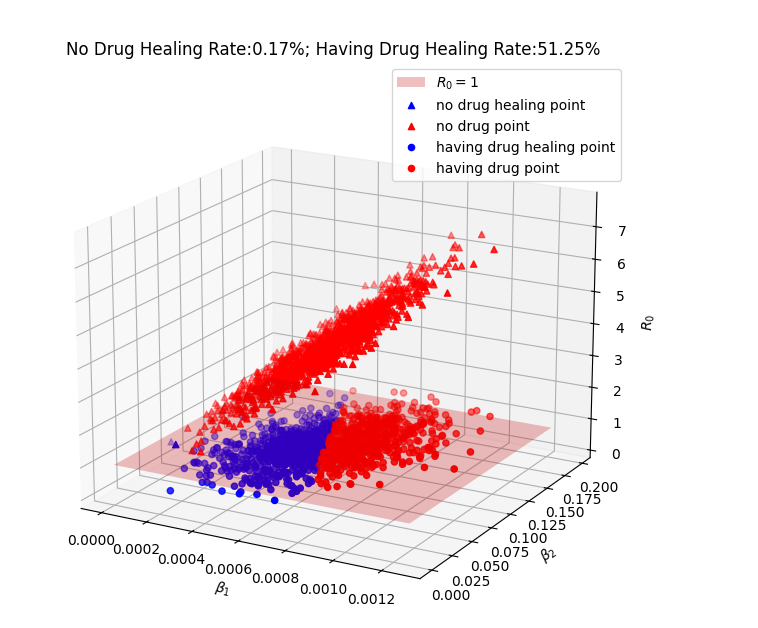
\includegraphics[width=0.8\linewidth]{6.2.1.png}
    \caption{自然条件下治愈率对比图($\varepsilon _{RT}=0.5,\varepsilon _{PI}=0.5$)}
    \label{fig.6.2.1}
\end{figure}
\begin{figure}[H]
    \centering
    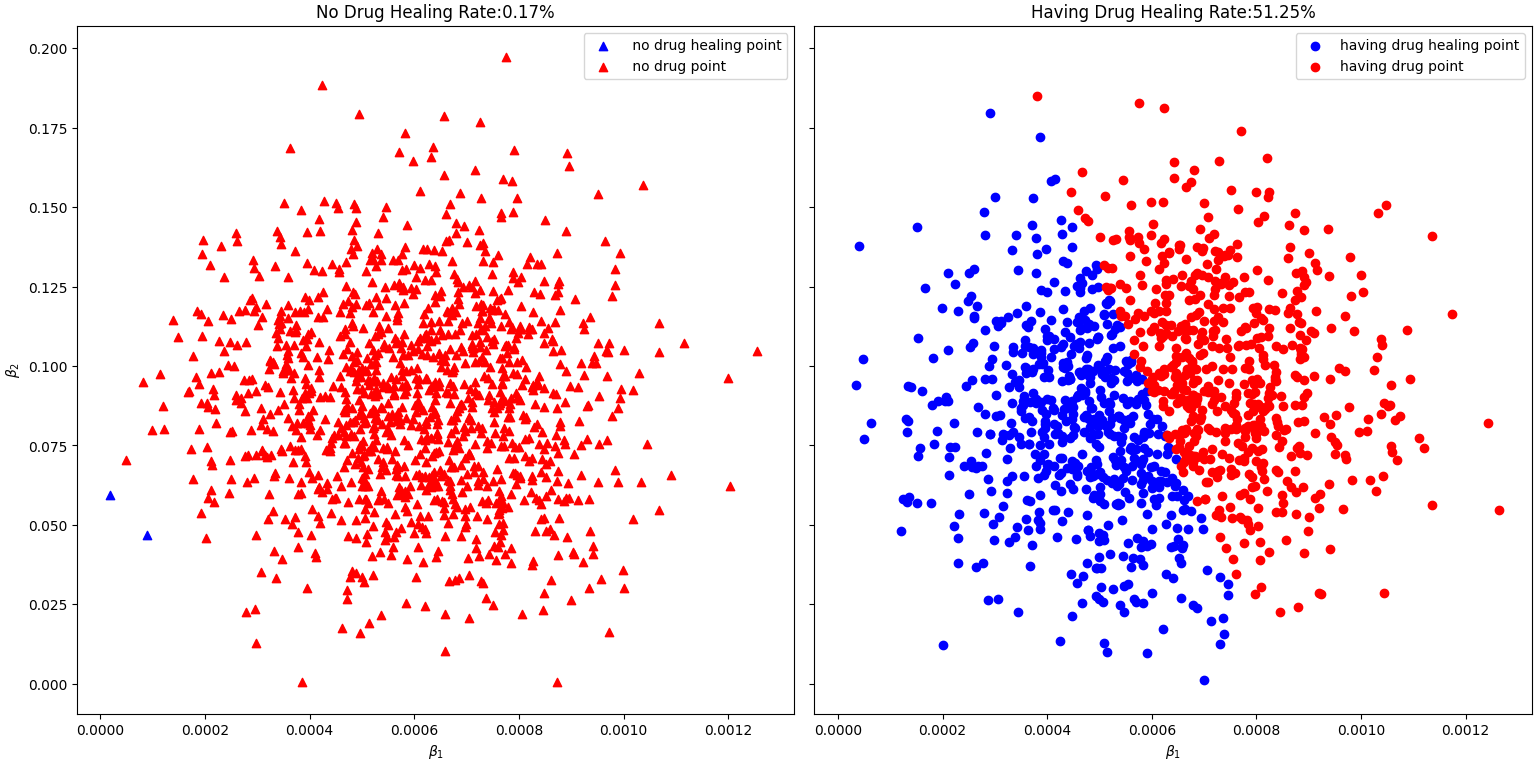
\includegraphics[width=\linewidth]{6.2.2.png}
    \caption{自然条件下治愈率对比图($\varepsilon _{RT}=0.5,\varepsilon _{PI}=0.5$)}
    \label{fig.6.2.2}
\end{figure}

\subsubsection{绘制自然条件下治愈率与药效关系图}
施加单种药物时药效的变化幅度为2.5\%,两种药物联合施加时各药的变化幅度为10\%。
\begin{figure}[H]
    \centering
    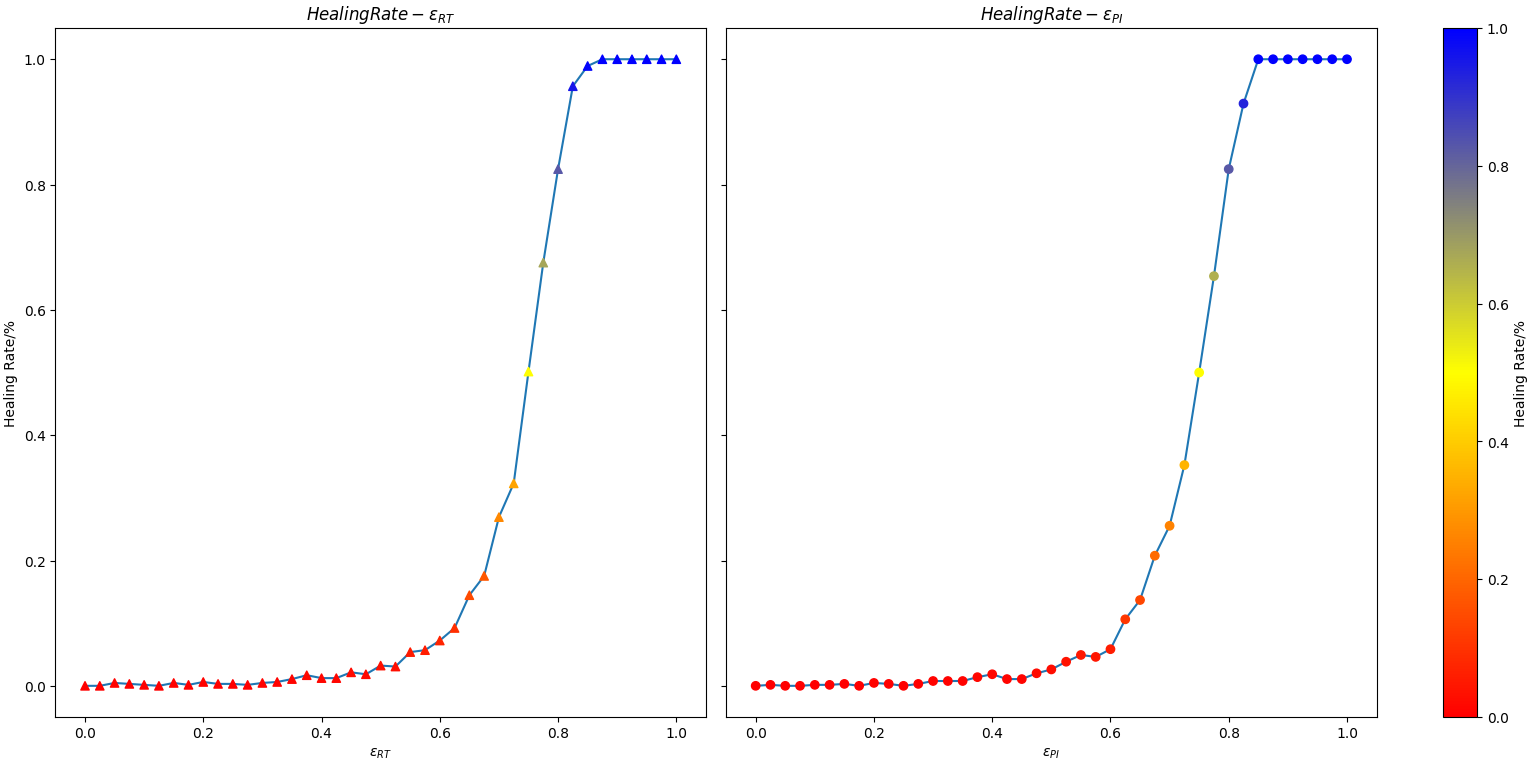
\includegraphics[width=\linewidth]{7.1.png}
    \caption{自然条件施加单种药物治愈率与药效关系图}
    \label{fig.7.1}
\end{figure}
\begin{figure}[H]
    \centering
    \begin{subfigure}[b]{0.49\linewidth}
        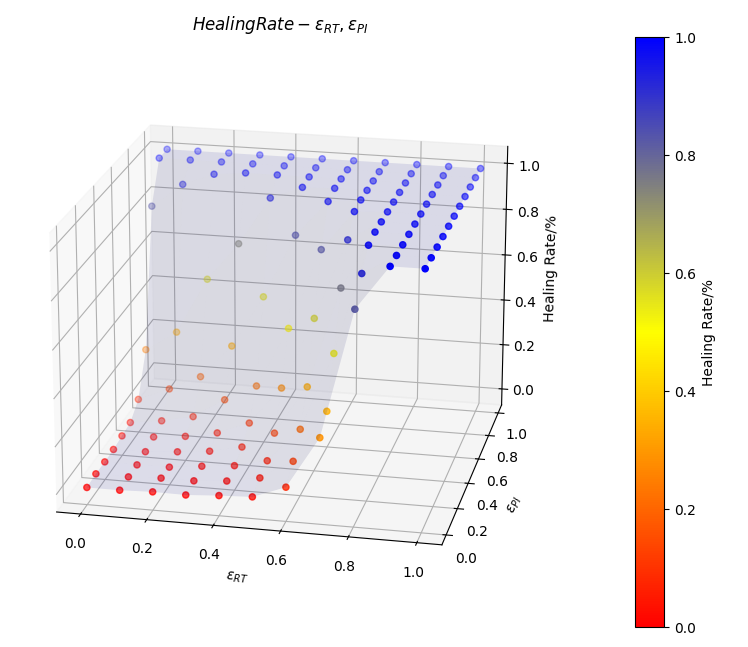
\includegraphics[width=\linewidth]{7.2.png}
        \caption{自然条件两种药物联合施加治愈率与药效关系图(3D)}
        \label{fig.7.2}
    \end{subfigure}
    \begin{subfigure}[b]{0.49\linewidth}
        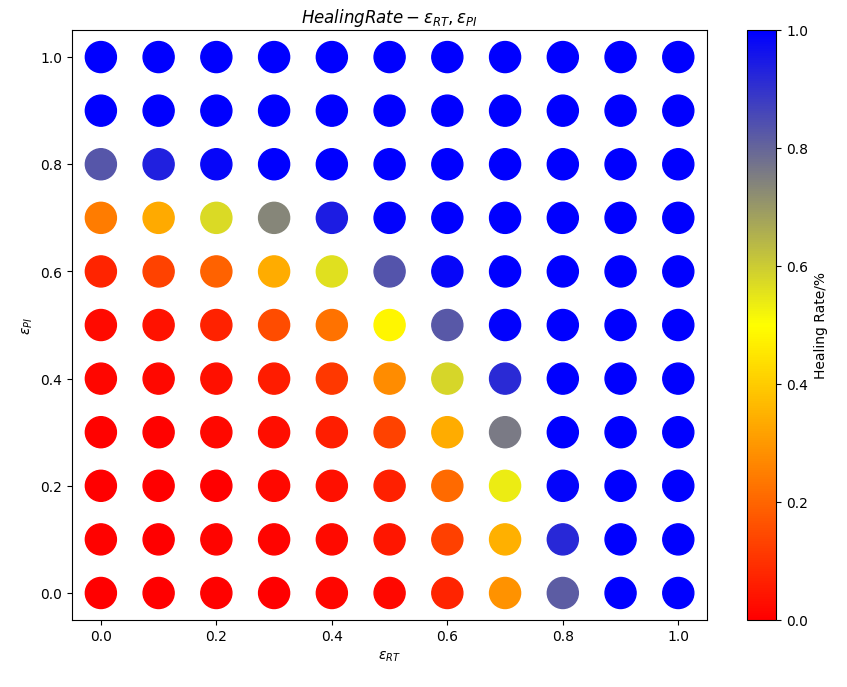
\includegraphics[width=\linewidth]{7.3.png}
        \caption{自然条件两种药物联合施加治愈率与药效关系图(2D)}
        \label{fig.7.3}
    \end{subfigure}
    \caption{自然条件两种药物联合施加治愈率与药效关系图}
    \label{fig.7.2-3}
\end{figure}

\section{学习心得和收获}
一个学期的python学习,我所获颇丰。在学习本课程前,我对python已经略有涉猎,但那时对python的认识非常肤浅,认为其仅比C语言语法简单(要求比较宽松)再便是可以绘图(这也是自学python的目的)。但进过一个学期系统地学习后,我才渐渐了解到python也有其自身的语法规范,python的变量类型并非我从前所认为的可以随便改变,列表、字典、数组看似相同但实际的结构和功能千差万别。在梳理清楚这些变量类型的同时也让我见识到了python的强大,以列表为例,切块、排序、寻找特殊值索引这些在C语言中比较繁琐的操作,在python列表中自带可以实现的方法,极大地简化了代码的编写。同时列表的.append()方法和字典无需提前设定内存大小可以随时添加,均为未知大小的数据的运算提供了便利。同时我还认识到了系统性学习的重要性,以类和对象的学习为例。在我刚刚接触python的时候便经常见到python是面向对象的编程,但是在网上碎片化学习的过程中一直无法理清类与对象的关系以其的作用,直到课堂上从概念开始,通过几个创建类、实例化为对象并调用类方法的例子,我才对类与对象有了基本概念,而实验课作业的实操帮助我巩固了基础概念加深了理解。这也让我意识到了及时复习和实际运用的重要性,感觉本学期的实验课作业形式对于非专业学生十分友好,恰如其分的提示极大地节省了我们理解问题的时间,可以更多地将精力放在python代码上,通过作业巩固每章的知识概念。python的学习还助力了我的科研,我是生物科学专业分子生物学方向,平时经常需要计算酶反应体系、PCR引物设计和基因序列(ATCG序列)比对,这些都是些耗时耗力的机械化操作,python对于字符串的便捷操作让我可以写一些小程序来完成这些简单重复劳动,节约了我的时间精力。这些基础知识的学习也为未来利用python对实验数据进行机器学习甚至是搭建神经网络奠定了基础。

\bibliographystyle{unsrt}
\bibliography{ref}


\end{document}
